% Capitolul 5: Modele ARCH/GARCH pentru Volatilitate
% Prezentare academică de calitate Harvard
% Program de licență, Academia de Studii Economice din București

\documentclass[9pt, aspectratio=169, t]{beamer}

% Asigură încadrarea conținutului pe diapozitive
\setbeamersize{text margin left=8mm, text margin right=8mm}

%=============================================================================
% CONFIGURARE TEMĂ ȘI STIL
%=============================================================================
\usetheme{default}
% Utilizăm tema implicită pentru control curat al antetului/subsolului

% Paletă de Culori (potrivită cu PDF-ul Redispatch)
\definecolor{MainBlue}{RGB}{26, 58, 110}
\definecolor{AccentBlue}{RGB}{26, 58, 110}
\definecolor{IDAred}{RGB}{205, 0, 0}
\definecolor{DarkGray}{RGB}{51, 51, 51}
\definecolor{MediumGray}{RGB}{128, 128, 128}
\definecolor{LightGray}{RGB}{248, 248, 248}
\definecolor{VeryLightGray}{RGB}{235, 235, 235}
\definecolor{KeynoteGray}{RGB}{218, 218, 218}
\definecolor{SectionGray}{RGB}{120, 120, 120}
\definecolor{FooterGray}{RGB}{100, 100, 100}
\definecolor{Crimson}{RGB}{220, 53, 69}
\definecolor{Forest}{RGB}{46, 125, 50}
\definecolor{Amber}{RGB}{181, 133, 63}
\definecolor{Orange}{RGB}{230, 126, 34}
\definecolor{Purple}{RGB}{142, 68, 173}

% Fundal gradient (gradient Keynote exact 315°: alb la RGB 218,218,218)
\setbeamertemplate{background}{%
    \begin{tikzpicture}[remember picture, overlay]
        \shade[shading=axis, shading angle=315,
        top color=white, bottom color=KeynoteGray]
        (current page.south west) rectangle (current page.north east);
    \end{tikzpicture}%
}
% Culoare solidă de rezervă pentru compatibilitate
\setbeamercolor{background canvas}{bg=}

\setbeamercolor{palette primary}{bg=MainBlue, fg=white}
\setbeamercolor{palette secondary}{bg=MainBlue!85, fg=white}
\setbeamercolor{palette tertiary}{bg=MainBlue!70, fg=white}
\setbeamercolor{structure}{fg=MainBlue}
\setbeamercolor{title}{fg=IDAred}
\setbeamercolor{frametitle}{fg=IDAred, bg=}
\setbeamercolor{block title}{bg=MainBlue, fg=white}
\setbeamercolor{block body}{bg=VeryLightGray, fg=DarkGray}
\setbeamercolor{block title alerted}{bg=Crimson, fg=white}
\setbeamercolor{block body alerted}{bg=Crimson!8, fg=DarkGray}
\setbeamercolor{block title example}{bg=Forest, fg=white}
\setbeamercolor{block body example}{bg=Forest!8, fg=DarkGray}
\setbeamercolor{item}{fg=MainBlue}

% Culori subsol (suprascriu albastrul temei Madrid)
\setbeamercolor{author in head/foot}{fg=FooterGray, bg=}
\setbeamercolor{title in head/foot}{fg=FooterGray, bg=}
\setbeamercolor{date in head/foot}{fg=FooterGray, bg=}
\setbeamercolor{section in head/foot}{fg=FooterGray, bg=}
\setbeamercolor{subsection in head/foot}{fg=FooterGray, bg=}

% Stiluri marcatori (se aplică peste tot inclusiv în blocuri)
\setbeamertemplate{itemize item}{\color{MainBlue}$\boxdot$}
\setbeamertemplate{itemize subitem}{\color{MainBlue}$\blacktriangleright$}
\setbeamertemplate{itemize subsubitem}{\color{MainBlue}\tiny$\bullet$}
\setbeamertemplate{itemize/enumerate body begin}{\normalsize}
\setbeamertemplate{itemize/enumerate subbody begin}{\normalsize}

% Item spacing - compact style
\setlength{\leftmargini}{10pt}       % Level 1: minimal indent
\setlength{\leftmarginii}{10pt}      % Level 2: minimal additional indent
% Compact list spacing (zero extra space before/after lists in blocks)
\makeatletter
\def\@listi{\leftmargin\leftmargini \topsep 0pt \parsep 0pt \itemsep 0pt}
\def\@listii{\leftmargin\leftmarginii \topsep 0pt \parsep 0pt \itemsep 0pt}
\makeatother

\setbeamertemplate{navigation symbols}{}

%=============================================================================
% ANTET PERSONALIZAT
%=============================================================================
\setbeamertemplate{headline}{%
    \vskip10pt%
    \hbox to \paperwidth{%
        \hskip0.5cm%
        {\small\color{FooterGray}\renewcommand{\hyperlink}[2]{##2}\insertsectionhead}%
        \hfill%
        \textcolor{FooterGray}{\small\insertframenumber}%
        \hskip0.5cm%
    }%
    \vskip4pt%
    {\color{FooterGray}\hrule height 0.4pt}%
}

%=============================================================================
% CUSTOM FOOTER
%=============================================================================
\usepackage{fontawesome5}

\setbeamertemplate{footline}{%
    {\color{FooterGray}\hrule height 0.4pt}%
    \vskip4pt%
    \hbox to \paperwidth{%
        \hskip0.5cm%
        \textcolor{FooterGray}{\small Analiza și Prognoza Seriilor de Timp}%
        \hfill%
        \raisebox{-0.1em}{%
            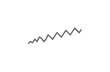
\begin{tikzpicture}[x=0.08em, y=0.08em, line width=0.4pt]
                \draw[FooterGray] (0,3) -- (1,4) -- (2,3.5) -- (3,5) -- (4,4) -- (5,6) -- (6,5.5) -- (7,4) -- (8,5) -- (9,7) -- (10,6) -- (11,5) -- (12,6.5) -- (13,8) -- (14,7) -- (15,6) -- (16,7.5) -- (17,9) -- (18,8) -- (19,7) -- (20,8.5) -- (21,10) -- (22,9) -- (23,8) -- (24,9.5);
            \end{tikzpicture}%
        }%
        \hskip0.5cm%
    }%
    \vskip6pt%
}

%=============================================================================
% PACHETE
%=============================================================================
\usepackage[utf8]{inputenc}
\usepackage[T1]{fontenc}
\usepackage{amsmath, amssymb, amsthm}
\usepackage{mathtools}
\usepackage{bm}
\usepackage{tikz}
\usetikzlibrary{arrows.meta, positioning, shapes, calc, decorations.pathreplacing, shadings}
\usepackage{booktabs}
\usepackage{multirow}
\usepackage{array}
\usepackage{graphicx}
\usepackage{hyperref}
\usepackage{colortbl}
\usepackage{listings}
\lstset{basicstyle=\ttfamily\small, breaklines=true, frame=single, backgroundcolor=\color{VeryLightGray}}
\hypersetup{colorlinks=true, linkcolor=MainBlue, urlcolor=MainBlue}
\graphicspath{{../../logos/}{../../charts/}{../../photos/}}
\hfuzz=2pt  % Suppress tiny overfull warnings (<2pt)
\vfuzz=2pt  % Suppress tiny vertical overfull warnings (<2pt)

%=============================================================================
% COMANDA QUANTLET
%=============================================================================
\newcommand{\quantlet}[2]{%
    \hfill\href{#2}{%
        \raisebox{-0.15em}{\includegraphics[height=0.7em]{ql_logo.png}}%
        \textcolor{MainBlue}{\tiny\ #1}%
    }%
}

%=============================================================================
% MEDII PENTRU TEOREME
%=============================================================================
\theoremstyle{definition}
\setbeamertemplate{theorems}[numbered]
\newtheorem{defn}{Definiție}
\newtheorem{thm}{Teoremă}
\newtheorem{prop}{Propoziție}
\newtheorem{rmk}{Observație}

%=============================================================================
% CENTRED MINIPAGE (fără spațiu vertical suplimentar)
%=============================================================================
\newenvironment{cminipage}[1]{%
    \par\noindent\hfill\begin{minipage}{#1}\ignorespaces
}{%
    \end{minipage}\hfill\null\par
}

%=============================================================================
% COMENZI PERSONALIZATE
%=============================================================================
\newcommand{\E}{\mathbb{E}}
\newcommand{\Var}{\text{Var}}
\newcommand{\Cov}{\text{Cov}}
\newcommand{\Corr}{\text{Corr}}
\newcommand{\R}{\mathbb{R}}
\newcommand{\N}{\mathbb{N}}
\newcommand{\Z}{\mathbb{Z}}
\newcommand{\B}{\mathbf{B}}
\newcommand{\imark}{\textcolor{MainBlue}{\textbullet}}
\newcommand{\RMSE}{\text{RMSE}}
\newcommand{\MAE}{\text{MAE}}
\newcommand{\MAPE}{\text{MAPE}}

%=============================================================================
% PAGINĂ TITLU PERSONALIZATĂ
%=============================================================================
\defbeamertemplate*{title page}{hybrid}[1][]
{
    \vspace{0.2cm}
    % Rând logo-uri - antet superior (cu linkuri clickabile)
    \begin{center}
        \href{https://www.ase.ro}{\includegraphics[height=1.0cm]{ase_logo.png}}\hspace{0.3cm}%
        \href{https://theida.net}{\includegraphics[height=1.0cm]{ida_logo.png}}\hspace{0.3cm}%
        \href{https://blockchain-research-center.com}{\includegraphics[height=1.0cm]{brc_logo.png}}\hspace{0.3cm}%
        \href{https://www.ai4efin.ase.ro}{\includegraphics[height=1.0cm]{ai4efin_logo.png}}\hspace{0.3cm}%
        \href{https://ipe.ro/new}{\includegraphics[height=1.0cm]{acad_logo.png}}\hspace{0.3cm}%
        \href{https://www.digital-finance-msca.com}{\includegraphics[height=1.0cm]{msca_logo.png}}%
    \end{center}

    \vspace{0.6cm}

    % Titlu principal cu logo-uri Q pe părți (cu linkuri clickabile)
    \begin{center}
        \begin{minipage}{0.1\textwidth}
            \centering
            \href{https://quantlet.com}{\includegraphics[height=1.1cm]{ql_logo.png}}
        \end{minipage}%
        \begin{minipage}{0.78\textwidth}
            \centering
            {\LARGE\bfseries\usebeamercolor[fg]{title}\inserttitle}

            \vspace{0.3cm}

            {\usebeamerfont{subtitle}\usebeamercolor[fg]{title}\insertsubtitle}
        \end{minipage}%
        \begin{minipage}{0.1\textwidth}
            \centering
            \href{https://quantinar.com}{\includegraphics[height=1.1cm]{qr_logo.png}}
        \end{minipage}
    \end{center}

    \vspace{0.6cm}

    % Autori (aliniere la stânga)
    \hspace{0.5cm}{\usebeamerfont{author}\insertauthor}

    \vspace{0.3cm}

    % Institut/Afilieri (aliniere la stânga)
    \hspace{0.5cm}\begin{minipage}[t]{0.9\textwidth}
        \raggedright\small\insertinstitute
    \end{minipage}
}

%=============================================================================
% INFORMAȚII TITLU
%=============================================================================
\title[Analiza Seriilor de Timp]{Analiza și Prognoza Seriilor de Timp}
\subtitle{Capitolul 5: Modele ARCH/GARCH pentru Volatilitate}
\author[D.T. Pele]{Daniel Traian PELE}
\institute{Academia de Studii Economice din București\\
IDA Institute Digital Assets\\
Blockchain Research Center\\
AI4EFin Artificial Intelligence for Energy Finance\\
Academia Română, Institutul de Prognoză Economică\\
MSCA Digital Finance}
\date{}

\begin{document}

% Pagina de titlu (fără antet/subsol)
{
\setbeamertemplate{headline}{}
\setbeamertemplate{footline}{}
\begin{frame}
    \titlepage
\end{frame}
}

%=============================================================================
% OBIECTIVE DE ÎNVĂȚARE
%=============================================================================
\section{Motivație}

\begin{frame}{Obiective de învățare}
    \begin{cminipage}{0.95\textwidth}
        \begin{block}{La finalul acestui capitol, veți fi capabili să:}
            \begin{enumerate}\setlength{\itemsep}{0pt}
                \item Înțelegeți \textbf{volatility clustering} și faptele stilizate ale randamentelor financiare
                \item Estimați și interpretați modele \textbf{ARCH} (Autoregressive Conditional Heteroskedasticity) și \textbf{GARCH} (Generalized ARCH)
                \item Aplicați modele asimetrice (\textbf{EGARCH} --- Exponential GARCH, \textbf{GJR-GARCH} --- Glosten-Jagannathan-Runkle) pentru efectul de levier
                \item Efectuați validarea și selectarea modelelor
                \item Prognozați volatilitatea și calculați \textbf{Value at Risk (VaR)}
            \end{enumerate}
        \end{block}
        \vspace{-0.1cm}
        \begin{alertblock}{Competențe practice}
            \begin{itemize}\setlength{\itemsep}{0pt}
                \item Implementare Python cu pachetul \texttt{arch}
                    \begin{itemize}\setlength{\itemsep}{0pt}
                        \item Estimare, prognoză și diagnostic automat
                    \end{itemize}
                \item Interpretarea parametrilor și a persistenței volatilității
                \item Calculul VaR pentru managementul riscului
                    \begin{itemize}\setlength{\itemsep}{0pt}
                        \item Backtesting și validarea prognozelor
                    \end{itemize}
            \end{itemize}
        \end{alertblock}
    \end{cminipage}
\end{frame}

%=============================================================================
% CUPRINS
%=============================================================================
\begin{frame}{Cuprins}
    \vspace{-0.3cm}
    {\small
    \begin{columns}[T]
        \begin{column}{0.48\textwidth}
            \begin{block}{Fundamente}
                \begin{itemize}\setlength{\itemsep}{3pt}
                    \item Motivație
                    \item Introducere în Modelarea Volatilității
                    \item Modelul ARCH
                    \item Modelul GARCH
                    \item Modele GARCH Asimetrice
                    \item Selectarea și Diagnosticarea modelelor
                \end{itemize}
            \end{block}
        \end{column}
        \begin{column}{0.48\textwidth}
            \begin{exampleblock}{Aplicații}
                \begin{itemize}\setlength{\itemsep}{3pt}
                    \item Prognoza volatilității
                    \item Implementare în Python
                    \item Studiu de Caz: S\&P 500
                    \item Studiu de Caz: Bitcoin
                    \item Rezumat și Quiz
                \end{itemize}
            \end{exampleblock}
        \end{column}
    \end{columns}
    }
\end{frame}

%=============================================================================
% SECȚIUNEA 1: INTRODUCERE ÎN MODELAREA VOLATILITĂȚII
%=============================================================================
\section{Introducere în Modelarea Volatilității}

\begin{frame}{Volatility clustering}
    \vspace{-0.2cm}
    {\scriptsize
    \begin{itemize}\setlength{\itemsep}{0pt}
        \item Perioadele de volatilitate mare sunt urmate de perioade de volatilitate mare; calm de calm
        \item Acest lucru sugerează că \textbf{varianța condiționată} este predictibilă
    \end{itemize}
    }
    \begin{center}
        \includegraphics[width=0.95\textwidth, height=0.50\textheight, keepaspectratio]{garch_volatility_clustering.pdf}
    \end{center}
    \quantlet{TSA\_ch5\_clustering}{https://github.com/QuantLet/TSA/tree/main/TSA_ch5/TSA_ch5_clustering}
\end{frame}

\begin{frame}{De ce modelăm volatilitatea?}
    \begin{cminipage}{0.95\textwidth}
        \small
        \begin{block}{Observații empirice în seriile financiare}
            \begin{itemize}\setlength{\itemsep}{0pt}
                \item Randamentele prezintă \textbf{volatility clustering} --- perioadele de volatilitate ridicată sunt urmate de perioade similare
                \item Distribuția randamentelor are \textbf{cozi groase} (leptokurtosis)
                \item Corelația randamentelor $\approx 0$, dar corelația pătratelor este semnificativă
                \item Volatilitatea răspunde \textbf{asimetric} la șocuri (leverage effect)
            \end{itemize}
        \end{block}

        \vspace{0.3cm}

        \begin{alertblock}{Limitarea modelelor ARIMA (Autoregressive Integrated Moving Average)}
            \begin{itemize}\setlength{\itemsep}{0pt}
                \item Modelele ARIMA presupun \textbf{varianță constantă} (homoscedasticitate)
                \item Această presupunere nu este realistă pentru seriile financiare!
            \end{itemize}
        \end{alertblock}
    \end{cminipage}
\end{frame}

\begin{frame}{Exemplu: Bitcoin $\succ$ volatility clustering}
    \begin{cminipage}{0.95\textwidth}
        {\small
        \begin{block}{Observații}
            \begin{itemize}\setlength{\itemsep}{0pt}
                \item Randamente zilnice Bitcoin (2019--2025): volatility clustering extrem de pronunțat
                    \begin{itemize}\setlength{\itemsep}{0pt}
                        \item Randamente de $\pm 20\%$ în perioadele de criză (COVID, Terra/Luna)
                    \end{itemize}
                \item Volatilitatea Bitcoin este semnificativ mai mare decât a activelor tradiționale
                    \begin{itemize}\setlength{\itemsep}{0pt}
                        \item $\alpha$ tipic $\approx 0.10$--$0.20$ (reacție rapidă la informații noi)
                    \end{itemize}
            \end{itemize}
        \end{block}
        }
    \end{cminipage}
\end{frame}

\begin{frame}{Exemplu: Bitcoin $\succ$ volatility clustering}
    \begin{center}
        \includegraphics[width=0.95\textwidth, height=0.78\textheight, keepaspectratio]{btc_returns.pdf}
    \end{center}
    \quantlet{TSA\_ch5\_btc\_returns}{https://github.com/QuantLet/TSA/tree/main/TSA_ch5/TSA_ch5_btc_returns}
\end{frame}

\begin{frame}{Fapte stilizate ale randamentelor financiare}
    \vspace{-0.2cm}
    {\scriptsize
    \begin{block}{Proprietăți observate}
        \begin{itemize}\setlength{\itemsep}{0pt}
            \item \textbf{Absența autocorelației} în randamente
                \begin{itemize}\setlength{\itemsep}{0pt}
                    \item $\text{Corr}(r_t, r_{t-k}) \approx 0$ --- randamentele sunt impredictibile
                \end{itemize}
            \item \textbf{Autocorelație} în $r_t^2$, $|r_t|$
                \begin{itemize}\setlength{\itemsep}{0pt}
                    \item $\text{Corr}(r_t^2, r_{t-k}^2) > 0$ --- volatilitatea este predictibilă
                \end{itemize}
            \item \textbf{Cozi groase} (kurtosis $> 3$)
                \begin{itemize}\setlength{\itemsep}{0pt}
                    \item Mai multe valori extreme decât prevede distribuția normală
                \end{itemize}
            \item \textbf{Leverage effect}
                \begin{itemize}\setlength{\itemsep}{0pt}
                    \item Șocurile negative cresc volatilitatea mai mult decât cele pozitive
                \end{itemize}
            \item \textbf{Volatility clustering}
                \begin{itemize}\setlength{\itemsep}{0pt}
                    \item Perioadele de volatilitate mare sunt urmate de volatilitate mare
                \end{itemize}
        \end{itemize}
    \end{block}
    }
\end{frame}

\begin{frame}{Fapte stilizate ale randamentelor financiare}
    \begin{center}
        \includegraphics[width=0.95\textwidth, height=0.78\textheight, keepaspectratio]{garch_stylized_facts.pdf}
    \end{center}
    \quantlet{TSA\_ch5\_stylized}{https://github.com/QuantLet/TSA/tree/main/TSA_ch5/TSA_ch5_stylized}
\end{frame}

\begin{frame}{Exemplu: Bitcoin $\succ$ evidență pentru efecte ARCH}
    \vspace{-0.2cm}
    {\scriptsize
    \begin{block}{Interpretare}
        \begin{itemize}\setlength{\itemsep}{0pt}
            \item ACF($r_t^2$) este semnificativ la multe lag-uri $\succ$ \textbf{efecte ARCH prezente}
            \item Varianța condiționată este predictibilă $\succ$ modelele GARCH sunt justificate
        \end{itemize}
    \end{block}
    }
    \begin{center}
        \includegraphics[width=0.95\textwidth, height=0.55\textheight, keepaspectratio]{btc_acf_squared.pdf}
    \end{center}
    \quantlet{TSA\_ch5\_btc\_arch}{https://github.com/QuantLet/TSA/tree/main/TSA_ch5/TSA_ch5_btc_arch}
\end{frame}

\begin{frame}{Heteroscedasticitate condiționată}
    \begin{cminipage}{0.95\textwidth}
        \small
        \begin{defn}[Varianță Condiționată]
            Pentru o serie de randamente $\{r_t\}$, \textbf{varianța condiționată} la momentul $t$ este:
            $\sigma_t^2 = \Var(r_t | \mathcal{F}_{t-1}) = \E[(r_t - \mu_t)^2 | \mathcal{F}_{t-1}]$
            unde $\mathcal{F}_{t-1}$ reprezintă informația disponibilă până la momentul $t-1$.
        \end{defn}

        \vspace{0.3cm}

        \begin{block}{Modelul general}
            $r_t = \mu_t + \varepsilon_t$, \quad $\varepsilon_t = \sigma_t z_t$, \quad $z_t \sim \text{i.i.d.}(0, 1)$
            \begin{itemize}\setlength{\itemsep}{0pt}
                \item $\mu_t$ = media condiționată (ARMA); \quad $\sigma_t^2$ = varianța condiționată (GARCH)
                \item $z_t$ = inovații standardizate (Normal, Student-t, GED --- Generalized Error Distribution)
            \end{itemize}
        \end{block}
    \end{cminipage}
\end{frame}

%=============================================================================
% SECȚIUNEA 2: MODELUL ARCH
%=============================================================================
\section{Modelul ARCH}

\begin{frame}{Portret de cercetător: Engle \& Bollerslev}
    \vspace{-0.2cm}
    \begin{columns}[T]
        \begin{column}{0.22\textwidth}
            \centering
            \includegraphics[width=0.95\textwidth, height=0.22\textheight, keepaspectratio]{photo_robert_engle.jpg}
            \\[0.05cm]
            {\tiny\textcolor{MediumGray}{Robert Engle (*1942)}}\\[-0.05cm]
            {\tiny\textcolor{MediumGray}{Premiul Nobel 2003}}\\[0.02cm]
            \href{https://en.wikipedia.org/wiki/Robert_F._Engle}{\faWikipediaW\ \textcolor{MainBlue}{\tiny Wikipedia (en)}}
        \end{column}
        \begin{column}{0.76\textwidth}
            \begin{block}{Biografie}
                {\footnotesize \begin{itemize}\setlength{\itemsep}{0pt}
                    \item \textbf{Robert Engle}: economist american la NYU Stern. Premiul Nobel (2003) ,,pentru metode de analiză a seriilor economice cu volatilitate variabilă în timp (ARCH)''
                    \item \textbf{Tim Bollerslev}: economist danez-american la Duke University, doctorand al lui Engle
                \end{itemize}}
            \end{block}
        \end{column}
    \end{columns}
    \vspace{0.1cm}
    \begin{columns}[T]
        \begin{column}{0.22\textwidth}
            \centering
            \includegraphics[width=0.95\textwidth, height=0.22\textheight, keepaspectratio]{photo_tim_bollerslev.jpg}
            \\[0.05cm]
            {\tiny\textcolor{MediumGray}{Tim Bollerslev (*1958)}}\\[0.02cm]
            \href{https://en.wikipedia.org/wiki/Tim_Bollerslev}{\faWikipediaW\ \textcolor{MainBlue}{\tiny Wikipedia (en)}}
        \end{column}
        \begin{column}{0.76\textwidth}
            \begin{exampleblock}{Contribuții principale}
                {\footnotesize
                \begin{itemize}\setlength{\itemsep}{0pt}
                    \item \textbf{Modelul ARCH} (Engle, 1982) --- heteroskedasticitate condiționată autoregresivă
                    \item \textbf{Modelul GARCH} (Bollerslev, 1986) --- ARCH generalizat cu volatilitate persistentă
                    \item \textbf{Volatilitatea realizată} și econometria de înaltă frecvență
                    \item Fundamentul managementului modern al riscului financiar (VaR, ES --- Expected Shortfall)
                \end{itemize}}
            \end{exampleblock}
        \end{column}
    \end{columns}
\end{frame}

\begin{frame}{Simulare ARCH(1): Efectul parametrului $\alpha$}
    \vspace{-0.2cm}
    {\small
    \begin{block}{Interpretare}
        \begin{itemize}\setlength{\itemsep}{0pt}
            \item Cu cât $\alpha$ este mai mare, cu atât volatilitatea reacționează mai puternic la șocuri recente
        \end{itemize}
    \end{block}
    }
    \begin{center}
        \includegraphics[width=0.95\textwidth, height=0.58\textheight, keepaspectratio]{garch_arch1_simulation.pdf}
    \end{center}
    \quantlet{TSA\_ch5\_arch\_sim}{https://github.com/QuantLet/TSA/tree/main/TSA_ch5/TSA_ch5_arch_sim}
\end{frame}

\begin{frame}{Modelul ARCH(q) --- Engle (1982)}
    \begin{cminipage}{0.95\textwidth}
        \small
        \begin{defn}[ARCH(q)]
            Modelul \textbf{Autoregressive Conditional Heteroskedasticity} de ordin $q$:
            \[
                \varepsilon_t = \sigma_t z_t, \quad z_t \sim \text{i.i.d.}(0, 1), \quad
                \sigma_t^2 = \omega + \sum_{i=1}^{q} \alpha_i \varepsilon_{t-i}^2
            \]
        \end{defn}

        \vspace{0.2cm}

        \begin{block}{Restricții pentru staționaritate}
            \begin{itemize}\setlength{\itemsep}{0pt}
                \item $\omega > 0$ (nivel de bază pozitiv), \quad $\alpha_i \geq 0$ (non-negativitate)
                \item $\sum_{i=1}^{q} \alpha_i < 1$ (staționaritate)
            \end{itemize}
        \end{block}
    \end{cminipage}
\end{frame}

\begin{frame}{Proprietăți ale modelului ARCH(1)}
    \begin{cminipage}{0.95\textwidth}
        \begin{block}{ARCH(1): $\sigma_t^2 = \omega + \alpha_1 \varepsilon_{t-1}^2$}
            \begin{itemize}\setlength{\itemsep}{0pt}
                \item \textbf{Varianța necondiționată}: $\E[\varepsilon_t^2] = \dfrac{\omega}{1 - \alpha_1}$ (dacă $\alpha_1 < 1$)
                \item \textbf{Kurtosis}: $\kappa = 3 \cdot \dfrac{1 - \alpha_1^2}{1 - 3\alpha_1^2}$ (dacă $\alpha_1^2 < 1/3$)
                \item Kurtosis $> 3$ pentru $\alpha_1 > 0$ $\succ$ \textbf{cozi groase}!
            \end{itemize}
        \end{block}

        \vspace{0.3cm}

        \begin{exampleblock}{Exemplu numeric}
            \begin{itemize}\setlength{\itemsep}{0pt}
                \item Dacă $\omega = 0.0001$ și $\alpha_1 = 0.3$:
                    \begin{itemize}\setlength{\itemsep}{0pt}
                        \item Varianța necondiționată: $\sigma^2 = \frac{0.0001}{1 - 0.3} = 0.000143$
                        \item Kurtosis: $\kappa = 3 \cdot \frac{1 - 0.09}{1 - 0.27} = 3.74 > 3$
                    \end{itemize}
            \end{itemize}
        \end{exampleblock}
    \end{cminipage}
\end{frame}

%=============================================================================
% DEMONSTRAȚII
%=============================================================================

\begin{frame}{Demonstrație: varianța necondiționată ARCH(1)}
    \begin{cminipage}{0.95\textwidth}
        \begin{proof}[Demonstrație]
            Fie $\varepsilon_t = \sigma_t z_t$ cu $z_t \sim N(0,1)$ și $\sigma_t^2 = \omega + \alpha_1 \varepsilon_{t-1}^2$.

            \vspace{0.2cm}
            \textbf{Pasul 1}: Aplicăm speranța necondiționată:
            \[
                \E[\varepsilon_t^2] = \E[\sigma_t^2 z_t^2] = \E[\sigma_t^2] \cdot \E[z_t^2] = \E[\sigma_t^2]
            \]

            \textbf{Pasul 2}: Aplicăm speranța ecuației varianței:
            \[
                \E[\sigma_t^2] = \E[\omega + \alpha_1 \varepsilon_{t-1}^2] = \omega + \alpha_1 \E[\varepsilon_{t-1}^2]
            \]

            \textbf{Pasul 3}: Prin staționaritate, $\E[\varepsilon_t^2] = \E[\varepsilon_{t-1}^2] = \sigma^2$:
            \[
                \sigma^2 = \omega + \alpha_1 \sigma^2 \quad \Rightarrow \quad \sigma^2 (1 - \alpha_1) = \omega
            \]

            \textbf{Rezultat}: $\boxed{\sigma^2 = \dfrac{\omega}{1 - \alpha_1}}$ \quad (necesită $\alpha_1 < 1$ pentru staționaritate)
        \end{proof}
    \end{cminipage}
\end{frame}

\begin{frame}{Demonstrație: kurtosis ARCH(1)}
    \begin{cminipage}{0.95\textwidth}
        {\small
        Pentru $\varepsilon_t = \sigma_t z_t$ cu $z_t \sim N(0,1)$:

        \textbf{Pasul 1}: $\E[\varepsilon_t^4] = \E[\sigma_t^4] \cdot \E[z_t^4] = 3 \E[\sigma_t^4]$ \quad (deoarece $\E[z^4] = 3$)

        \textbf{Pasul 2}: Folosind $\sigma_t^2 = \omega + \alpha_1 \varepsilon_{t-1}^2$:
        \[
            \E[\sigma_t^4] = \E[(\omega + \alpha_1 \varepsilon_{t-1}^2)^2] = \omega^2 + 2\omega\alpha_1 \sigma^2 + \alpha_1^2 \E[\varepsilon_{t-1}^4]
        \]

        \textbf{Pasul 3}: Rezolvând recurența:
        \[
            \boxed{\kappa = \frac{\E[\varepsilon_t^4]}{(\E[\varepsilon_t^2])^2} = 3 \cdot \frac{1 - \alpha_1^2}{1 - 3\alpha_1^2}}
        \]
        }

        \begin{block}{Interpretare}
            \begin{itemize}\setlength{\itemsep}{0pt}
                \item $\kappa > 3$ pentru orice $\alpha_1 > 0$ $\succ$ \textbf{cozi groase} (leptokurtosis)
                \item Necesită $\alpha_1 < 0.577$ pentru moment de ordin 4 finit
                \item ARCH generează în mod natural distribuții cu cozi groase!
            \end{itemize}
        \end{block}
    \end{cminipage}
\end{frame}

\begin{frame}{Teorie vs empirică: decalajul kurtosis}
    \begin{cminipage}{0.95\textwidth}
        \small
        \vspace{-0.2cm}
        \begin{block}{Kurtosis ARCH(1): prea mică!}
            \begin{itemize}\setlength{\itemsep}{0pt}
                \item Pentru randamente tipice de acțiuni: $\alpha_1 \approx 0.09$ (S\&P 500)
                \item Kurtosis teoretică: $\kappa = 3 \cdot \frac{1 - 0.09^2}{1 - 3 \times 0.09^2} \approx \textbf{3.05}$
                \item Kurtosis empirică a randamentelor zilnice S\&P 500: $\kappa \approx \textbf{13.8}$
            \end{itemize}
        \end{block}
        \vspace{-0.1cm}
        \begin{alertblock}{Decalajul kurtosis}
            \begin{center}
            {\large $\underbrace{3.05}_{\text{ARCH(1)-Normal}} \;\ll\; \underbrace{13.8}_{\text{Empiric}}$}
            \end{center}
            \vspace{-2mm}
            \begin{itemize}\setlength{\itemsep}{0pt}
                \item ARCH(1) cu inovații gaussiene nu poate reproduce kurtosis-ul extrem observat în datele financiare
            \end{itemize}
        \end{alertblock}
        \vspace{-0.1cm}
        \begin{exampleblock}{Soluții}
            \begin{itemize}\setlength{\itemsep}{0pt}
                \item \textbf{Inovații Student-$t$}: $z_t \sim t_\nu$ adaugă kurtosis din distribuția însăși
                \item \textbf{GARCH(1,1)}: persistența ($\beta > 0$) generează kurtosis suplimentar
                \item Ambele combinate: Student-$t$ GARCH capturează $\kappa \gg 3$ observat în practică
            \end{itemize}
        \end{exampleblock}
    \end{cminipage}
\end{frame}

\begin{frame}{Testarea efectelor ARCH}
    \begin{cminipage}{0.95\textwidth}
        \begin{block}{Testul Engle pentru efecte ARCH}
            \textbf{Procedură}:
            \begin{enumerate}\setlength{\itemsep}{0pt}
                \item Estimează modelul pentru medie și obține reziduurile $\hat{\varepsilon}_t$
                \item Calculează $\hat{\varepsilon}_t^2$
                \item Regresează $\hat{\varepsilon}_t^2$ pe lag-urile sale:
                \[
                    \hat{\varepsilon}_t^2 = \beta_0 + \beta_1 \hat{\varepsilon}_{t-1}^2 + \cdots + \beta_q \hat{\varepsilon}_{t-q}^2 + u_t
                \]
                \item Calculează statistica $LM = T \cdot R^2 \sim \chi^2(q)$
            \end{enumerate}
        \end{block}

        \vspace{0.3cm}

        \begin{alertblock}{Ipoteze}
            \begin{itemize}\setlength{\itemsep}{0pt}
                \item $H_0$: Nu există efecte ARCH ($\alpha_1 = \cdots = \alpha_q = 0$)
                \item $H_1$: Există efecte ARCH (cel puțin un $\alpha_i \neq 0$)
            \end{itemize}
        \end{alertblock}
    \end{cminipage}
\end{frame}

\begin{frame}{Limitări ale modelului ARCH}
    \begin{cminipage}{0.95\textwidth}
        \begin{alertblock}{Probleme practice}
            \begin{enumerate}\setlength{\itemsep}{0pt}
                \item \textbf{Ordin mare} --- de obicei sunt necesare multe lag-uri ($q$ mare)
                \item \textbf{Mulți parametri} --- dificultăți de estimare
                \item \textbf{Restricții de non-negativitate} --- greu de impus pentru $q$ mare
                \item \textbf{Nu capturează persistența} --- volatilitatea observată este foarte persistentă
            \end{enumerate}
        \end{alertblock}

        \vspace{0.5cm}

        \begin{block}{Soluția}
            \begin{itemize}\setlength{\itemsep}{0pt}
                \item \textbf{Modelul GARCH} --- introduce lag-uri ale varianței condiționate pentru a captura persistența cu mai puțini parametri!
            \end{itemize}
        \end{block}
    \end{cminipage}
\end{frame}

%=============================================================================
% SECȚIUNEA 3: MODELUL GARCH
%=============================================================================
\section{Modelul GARCH}

\begin{frame}{Modelul GARCH(1,1)}
    \vspace{-0.2cm}
    \begin{cminipage}{0.95\textwidth}
        {\small
        \begin{block}{Cel mai popular model de volatilitate}
            \begin{itemize}\setlength{\itemsep}{0pt}
                \item $\sigma_t^2 = \omega + \alpha \varepsilon_{t-1}^2 + \beta \sigma_{t-1}^2$
            \end{itemize}
        \end{block}

        \vspace{0.2cm}

        \begin{block}{Restricții și proprietăți}
            \begin{itemize}\setlength{\itemsep}{0pt}
                \item $\omega > 0$, $\alpha \geq 0$, $\beta \geq 0$; \quad $\alpha + \beta < 1$ (staționaritate)
                \item $\bar{\sigma}^2 = \frac{\omega}{1 - \alpha - \beta}$; \quad Half-life: $HL = \frac{\ln(0.5)}{\ln(\alpha + \beta)}$
            \end{itemize}
        \end{block}
        }
    \end{cminipage}
\end{frame}

\begin{frame}{Modelul GARCH(1,1)}
    \begin{center}
        \includegraphics[width=0.95\textwidth, height=0.78\textheight, keepaspectratio]{garch_conditional_variance.pdf}
    \end{center}
\end{frame}

\begin{frame}{Modelul GARCH(p,q) --- Bollerslev (1986)}
    \begin{cminipage}{0.95\textwidth}
        \small
        \begin{defn}[GARCH(p,q)]
            Modelul \textbf{Generalized ARCH}:
            \[
                \varepsilon_t = \sigma_t z_t, \quad z_t \sim \text{i.i.d.}(0, 1)
            \]
            \[
                \sigma_t^2 = \omega + \sum_{i=1}^{q} \alpha_i \varepsilon_{t-i}^2 + \sum_{j=1}^{p} \beta_j \sigma_{t-j}^2
            \]
        \end{defn}

        \vspace{0.3cm}

        \begin{block}{Interpretare}
            \begin{itemize}\setlength{\itemsep}{0pt}
                \item $\omega$ = nivel de bază al volatilității
                \item $\alpha_i$ = reacția la șocuri recente (coeficienți de impact)
                \item $\beta_j$ = persistența volatilității (memorie)
                \item $\alpha + \beta$ = persistența totală
            \end{itemize}
        \end{block}
    \end{cminipage}
\end{frame}

\begin{frame}{Simulare GARCH(1,1): efectul persistenței}
    \vspace{-0.2cm}
    {\footnotesize
    \begin{block}{Interpretare}
        \begin{itemize}\setlength{\itemsep}{0pt}
            \item $\alpha$ controlează reacția la șocuri
            \item $\beta$ controlează persistența
            \item Suma $\alpha + \beta$ determină viteza de revenire la medie
        \end{itemize}
    \end{block}
    }
    \begin{center}
        \includegraphics[width=0.95\textwidth, height=0.50\textheight, keepaspectratio]{garch_garch11_simulation.pdf}
    \end{center}
    \quantlet{TSA\_ch5\_garch\_sim}{https://github.com/QuantLet/TSA/tree/main/TSA_ch5/TSA_ch5_garch_sim}
\end{frame}

\begin{frame}{Demonstrație: varianța necondiționată GARCH(1,1)}
    \small
    \begin{proof}[Demonstrație]
        Pentru $\sigma_t^2 = \omega + \alpha \varepsilon_{t-1}^2 + \beta \sigma_{t-1}^2$:

        \textbf{Pasul 1}: Aplicăm speranța necondiționată:
        $\E[\sigma_t^2] = \omega + \alpha \E[\varepsilon_{t-1}^2] + \beta \E[\sigma_{t-1}^2]$

        \textbf{Pasul 2}: Prin staționaritate, $\E[\sigma_t^2] = \E[\sigma_{t-1}^2] = \bar{\sigma}^2$ și $\E[\varepsilon_t^2] = \bar{\sigma}^2$:
        $\bar{\sigma}^2 = \omega + (\alpha + \beta) \bar{\sigma}^2$

        \textbf{Pasul 3}: Rezolvăm: $\bar{\sigma}^2 (1 - \alpha - \beta) = \omega \Rightarrow \boxed{\bar{\sigma}^2 = \frac{\omega}{1 - \alpha - \beta}}$
    \end{proof}
    \vspace{-0.1cm}
    \begin{alertblock}{Condiție de staționaritate}
        \begin{itemize}\setlength{\itemsep}{0pt}
            \item Necesită $\alpha + \beta < 1$ pentru varianță necondiționată finită
        \end{itemize}
    \end{alertblock}
\end{frame}

\begin{frame}{GARCH(1,1) ca ARMA pentru $\varepsilon_t^2$}
    \vspace{-0.2cm}
    {\footnotesize
    \begin{block}{Reprezentare ARMA(1,1)}
        \begin{itemize}\setlength{\itemsep}{0pt}
            \item Definim $\nu_t = \varepsilon_t^2 - \sigma_t^2$ (șocul varianței). Atunci:
            \[
                \varepsilon_t^2 = \omega + (\alpha + \beta) \varepsilon_{t-1}^2 + \nu_t - \beta \nu_{t-1}
            \]
            \item Aceasta este un \textbf{ARMA(1,1)} pentru $\varepsilon_t^2$!
        \end{itemize}
    \end{block}

    \vspace{0.3cm}

    \begin{exampleblock}{Implicații}
        \begin{itemize}\setlength{\itemsep}{0pt}
            \item ACF al $\varepsilon_t^2$ decade exponențial (ca ARMA)
            \item Persistența este dată de $\alpha + \beta$
            \item PACF poate ajuta la identificarea ordinului
        \end{itemize}
    \end{exampleblock}
    }
\end{frame}

\begin{frame}{Demonstrație: Reprezentarea ARMA a GARCH(1,1)}
    \begin{proof}[Demonstrație]
        \textbf{Pasul 1}: Definim șocul varianței: $\nu_t = \varepsilon_t^2 - \sigma_t^2$
        \begin{itemize}\setlength{\itemsep}{0pt}
            \item $\E[\nu_t | \mathcal{F}_{t-1}] = \E[\varepsilon_t^2 | \mathcal{F}_{t-1}] - \sigma_t^2 = \sigma_t^2 - \sigma_t^2 = 0$
            \item $\nu_t$ este o secvență diferență de martingal
        \end{itemize}

        \vspace{0.2cm}
        \textbf{Pasul 2}: Înlocuim $\sigma_t^2 = \varepsilon_t^2 - \nu_t$ în ecuația GARCH:
        \[
            \varepsilon_t^2 - \nu_t = \omega + \alpha \varepsilon_{t-1}^2 + \beta (\varepsilon_{t-1}^2 - \nu_{t-1})
        \]

        \textbf{Pasul 3}: Rearanjăm:
        \[
            \varepsilon_t^2 = \omega + (\alpha + \beta) \varepsilon_{t-1}^2 + \nu_t - \beta \nu_{t-1}
        \]

        \textbf{Rezultat}: ARMA(1,1) cu coeficient AR $\phi = \alpha + \beta$ și coeficient MA $\theta = -\beta$.
    \end{proof}
\end{frame}

\begin{frame}{Demonstrație: persistența volatilității și half-life}
    \begin{cminipage}{0.95\textwidth}
        \small
        \begin{block}{Prognoză multi-pas GARCH(1,1)}
            \begin{itemize}\setlength{\itemsep}{0pt}
                \item $\E_t[\sigma_{t+h}^2] = \bar{\sigma}^2 + (\alpha+\beta)^{h-1}(\sigma_{t+1}^2 - \bar{\sigma}^2)$
            \end{itemize}
        \end{block}
        \vspace{-0.1cm}
        \begin{block}{Demonstrație}
            \begin{itemize}\setlength{\itemsep}{0pt}
                \item \textbf{Pasul 1}: Notăm $\phi = \alpha + \beta$ și $q_t = \sigma_t^2 - \bar{\sigma}^2$ (deviația de la medie)
                \item \textbf{Pasul 2}: Din ecuația GARCH: $\E_t[q_{t+1}] = \phi \cdot q_t$, deci $\E_t[q_{t+h}] = \phi^h \cdot q_t$
                \item \textbf{Pasul 3}: Half-life = timpul până când deviația se înjumătățește:
                $\phi^{HL} = 0.5 \;\Rightarrow\; HL = \frac{\ln(0.5)}{\ln(\phi)} = \frac{-0.693}{\ln(\alpha+\beta)}$
            \end{itemize}
        \end{block}
        \vspace{-0.1cm}
        \begin{exampleblock}{Exemplu: S\&P 500}
            \begin{itemize}\setlength{\itemsep}{0pt}
                \item Cu $\alpha + \beta = 0.988$: $HL = \frac{-0.693}{-0.012} \approx \textbf{58 zile}$ (șocurile persistă $\sim$3 luni!)
            \end{itemize}
        \end{exampleblock}
    \end{cminipage}
\end{frame}

\begin{frame}{Estimarea modelelor GARCH}
    \begin{cminipage}{0.95\textwidth}
        \small
        \begin{block}{Metoda verosimilității maxime (MLE --- Maximum Likelihood Estimation)}
            \begin{itemize}\setlength{\itemsep}{0pt}
                \item Log-verosimilitate (normală): $\ell(\theta) = -\frac{T}{2} \ln(2\pi) - \frac{1}{2} \sum_{t=1}^{T} \left[ \ln(\sigma_t^2) + \frac{\varepsilon_t^2}{\sigma_t^2} \right]$
            \end{itemize}
        \end{block}

        \vspace{0.2cm}

        \begin{block}{Distribuții alternative pentru $z_t$}
            \begin{itemize}\setlength{\itemsep}{0pt}
                \item \textbf{Student-t}: capturează cozile groase --- cea mai frecventă alegere
                \item \textbf{GED}: flexibilitate pentru kurtosis
                \item \textbf{Skewed Student-t}: asimetrie și cozi groase
            \end{itemize}
        \end{block}

        \vspace{0.2cm}

        \begin{alertblock}{Notă practică}
            \begin{itemize}\setlength{\itemsep}{0pt}
                \item Distribuția Student-t oferă de regulă o potrivire mai bună pentru randamentele financiare datorită cozilor groase (kurtosis $> 3$)
            \end{itemize}
        \end{alertblock}
    \end{cminipage}
\end{frame}

\begin{frame}{Quasi-MLE și robustețe}
    \begin{cminipage}{0.95\textwidth}
        \scriptsize
        \setlength{\abovedisplayskip}{2pt}\setlength{\belowdisplayskip}{2pt}
        \vspace{-0.3cm}
        \begin{block}{Ce se întâmplă dacă distribuția este greșit specificată?}
            \begin{itemize}\setlength{\itemsep}{0pt}
                \item MLE standard presupune $z_t \sim N(0,1)$, dar distribuția reală poate diferi
                \item \textbf{Quasi-MLE (QMLE --- Quasi-Maximum Likelihood Estimation)}: maximizează log-verosimilitatea gaussiană chiar dacă $z_t$ nu este normal
                \item De remarcat: avem nevoie doar ca \textit{primele două momente condiționate} să fie corecte
            \end{itemize}
        \end{block}
        \vspace{-0.2cm}
        \begin{defn}[Consistența QMLE --- Bollerslev \& Wooldridge (1992)]
            \begin{itemize}\setlength{\itemsep}{0pt}
                \item Dacă media și varianța condiționate sunt corect specificate, QMLE este \textbf{consistent} pentru $(\omega, \alpha, \beta)$ indiferent de distribuția reală a lui $z_t$
            \end{itemize}
        \end{defn}
        \vspace{-0.2cm}
        \begin{alertblock}{Erori standard sandwich (robuste)}
            \begin{itemize}\setlength{\itemsep}{0pt}
                \item Erorile standard trebuie corectate:
                \[
                    \hat{V}_{\text{robust}} = \hat{A}^{-1} \hat{B} \hat{A}^{-1} \quad \text{(White, 1982)}
                \]
                \item $\hat{A}$ = Hessiana, $\hat{B}$ = produsul exterior al scorurilor
                \item În Python: \texttt{result.summary()} raportează SE robuste implicit
            \end{itemize}
        \end{alertblock}
        \vspace{-0.15cm}
        \begin{exampleblock}{Când folosim QMLE vs MLE complet}
            \begin{itemize}\setlength{\itemsep}{0pt}
                \item \textbf{QMLE}: implicit sigur --- consistent chiar sub specificare greșită
                \item \textbf{MLE complet} (Student-$t$): mai \textit{eficient} dacă distribuția este corectă
            \end{itemize}
        \end{exampleblock}
    \end{cminipage}
\end{frame}

\begin{frame}{Provocări practice în estimare}
    \begin{cminipage}{0.95\textwidth}
        \small
        \begin{block}{Probleme frecvente}
            \begin{itemize}\setlength{\itemsep}{0pt}
                \item \textbf{Eșec de convergență}: log-verosimilitatea este non-convexă; optimizatorul se poate bloca
                \item \textbf{Soluții la frontieră}: $\hat{\alpha} \approx 0$ sau $\hat{\alpha} + \hat{\beta} \approx 1$ (aproape IGARCH --- Integrated GARCH)
                \item \textbf{Sensibilitate la valori inițiale}: inițializări diferite $\succ$ estimări diferite
            \end{itemize}
        \end{block}
        \vspace{-0.1cm}
        \begin{exampleblock}{Bune practici}
            \begin{enumerate}\setlength{\itemsep}{0pt}
                \item Încercați mai mulți optimizatori: \textbf{BFGS} (rapid, bazat pe gradient) vs \textbf{Nelder-Mead} (fără derivate)
                \item Inițializați $\sigma_0^2$ cu varianța eșantionului (backcast)
                \item Verificați $\alpha + \beta < 1$ post-estimare; dacă $\approx 1$, considerați IGARCH sau schimbare de regim
                \item Comparați rezultatele între valori inițiale; estimări consistente $\succ$ model fiabil
            \end{enumerate}
        \end{exampleblock}
        \vspace{-0.1cm}
        \begin{alertblock}{Regulă practică}
            \begin{itemize}\setlength{\itemsep}{0pt}
                \item Dacă BFGS și Nelder-Mead dau estimări \textit{diferite} ale parametrilor, modelul poate fi greșit specificat sau datele insuficiente
            \end{itemize}
        \end{alertblock}
    \end{cminipage}
\end{frame}

\begin{frame}{Valori tipice pentru GARCH(1,1)}
    \begin{cminipage}{0.95\textwidth}
        \begin{center}
            \begin{tabular}{lccc}
                \toprule
                \textbf{Serie} & $\bm{\alpha}$ & $\bm{\beta}$ & $\bm{\alpha + \beta}$ \\
                \midrule
                S\&P 500 zilnic & 0.05--0.10 & 0.85--0.95 & 0.95--0.99 \\
                EUR/USD zilnic & 0.03--0.08 & 0.90--0.95 & 0.95--0.99 \\
                Bitcoin zilnic & 0.10--0.20 & 0.75--0.85 & 0.90--0.98 \\
                Obligațiuni & 0.02--0.05 & 0.90--0.97 & 0.95--0.99 \\
                \bottomrule
            \end{tabular}
        \end{center}

        \vspace{0.5cm}

        \begin{alertblock}{Observații}
            \begin{itemize}\setlength{\itemsep}{0pt}
                \item $\alpha + \beta$ aproape de 1 $\succ$ \textbf{volatilitate foarte persistentă}
                \item $\alpha$ mic, $\beta$ mare $\succ$ reacție lentă la șocuri, memorie lungă
                \item Bitcoin: $\alpha$ mai mare $\succ$ reacție mai rapidă la informații noi
            \end{itemize}
        \end{alertblock}
    \end{cminipage}
\end{frame}

\begin{frame}{GARCH vs IGARCH: comparație persistență}
    \vspace{-0.2cm}
    {\scriptsize
    \begin{block}{Interpretare}
        \begin{itemize}\setlength{\itemsep}{0pt}
            \item GARCH standard revine la media necondiționată
            \item IGARCH nu are medie finită $\succ$ șocurile persistă indefinit
        \end{itemize}
    \end{block}
    }
    \begin{center}
        \includegraphics[width=0.95\textwidth, height=0.50\textheight, keepaspectratio]{garch_igarch_comparison.pdf}
    \end{center}
    \quantlet{TSA\_ch5\_igarch}{https://github.com/QuantLet/TSA/tree/main/TSA_ch5/TSA_ch5_igarch}
\end{frame}

\begin{frame}{IGARCH --- integrated GARCH}
    \begin{cminipage}{0.95\textwidth}
        \small
        \begin{defn}[IGARCH(1,1)]
            Când $\alpha + \beta = 1$:
            \[
                \sigma_t^2 = \omega + \alpha \varepsilon_{t-1}^2 + (1 - \alpha) \sigma_{t-1}^2
            \]
        \end{defn}

        \vspace{0.3cm}

        \begin{block}{Proprietăți}
            \begin{itemize}\setlength{\itemsep}{0pt}
                \item Varianța necondiționată nu există (infinită)
                \item Șocurile au efect \textbf{permanent} asupra volatilității
                \item Folosit pentru serii cu persistență extremă
                \item Util pentru \textbf{RiskMetrics} (J.P. Morgan): $\alpha = 0.06$, $\beta = 0.94$
            \end{itemize}
        \end{block}

        \begin{rmk}
            \begin{itemize}\setlength{\itemsep}{0pt}
                \item IGARCH este analog cu o rădăcină unitară în varianță!
            \end{itemize}
        \end{rmk}
    \end{cminipage}
\end{frame}

\begin{frame}{Schimbări de regim în volatilitate}
    \begin{cminipage}{0.95\textwidth}
        \scriptsize
        \setlength{\abovedisplayskip}{2pt}\setlength{\belowdisplayskip}{2pt}
        \vspace{-0.3cm}
        \begin{block}{Problemă}
            \begin{itemize}\setlength{\itemsep}{0pt}
                \item GARCH presupune un \textbf{singur regim} cu parametri constanți
                \item Volatilitatea prezintă adesea \textbf{rupturi structurale} (ex.\ criza 2008, COVID-19)
            \end{itemize}
        \end{block}
        \vspace{-0.2cm}
        \begin{defn}[GARCH cu schimbare de regim Markov]
            Parametrii $(\omega, \alpha, \beta)$ comută între $K$ regimuri guvernate de un lanț Markov ascuns:
            \[
                \sigma_t^2 = \omega_{s_t} + \alpha_{s_t} \varepsilon_{t-1}^2 + \beta_{s_t} \sigma_{t-1}^2, \quad s_t \in \{1, \ldots, K\}
            \]
        \end{defn}
        \vspace{-0.2cm}
        \begin{exampleblock}{Testul ICSS (Iterated Cumulative Sums of Squares) --- Inclán-Tiao}
            \begin{itemize}\setlength{\itemsep}{0pt}
                \item Detectează \textbf{puncte de schimbare multiple} în varianța necondiționată
                \item Bazat pe suma cumulativă a observațiilor pătrate (tip CUSUM)
                \item Rezultate tipice: S\&P 500 arată rupturi la 2001, 2008, 2020
            \end{itemize}
        \end{exampleblock}
        \vspace{-0.2cm}
        \begin{alertblock}{Implicații practice}
            \begin{itemize}\setlength{\itemsep}{0pt}
                \item Dacă rupturile sunt prezente, persistența GARCH ($\alpha + \beta$) este \textbf{biasată în sus} $\succ$ IGARCH spurios
                \item Soluție: estimare GARCH separată per regim, sau ferestre rulante
                \item Alternativă: GARCH cu schimbare Markov cu $K=2$ (regim volatilitate scăzută / ridicată)
            \end{itemize}
        \end{alertblock}
    \end{cminipage}
\end{frame}

%=============================================================================
% SECȚIUNEA 4: MODELE GARCH ASIMETRICE
%=============================================================================
\section{Modele GARCH Asimetrice}

\begin{frame}{Leverage effect}
    \begin{cminipage}{0.95\textwidth}
        {\scriptsize
        \begin{block}{Definiție}
            \begin{itemize}\setlength{\itemsep}{0pt}
                \item \textbf{Leverage effect}: Șocurile negative cresc volatilitatea \textbf{mai mult} decât cele pozitive de aceeași magnitudine
            \end{itemize}
        \end{block}
        \begin{alertblock}{Problema GARCH standard}
            \begin{itemize}\setlength{\itemsep}{0pt}
                \item GARCH standard: $\sigma_t^2 = \omega + \alpha \varepsilon_{t-1}^2 + \beta \sigma_{t-1}^2$ --- doar $\varepsilon_{t-1}^2$ contează, semnul se pierde!
                \item Intuiție economică: Vești proaste $\succ$ prețul scade $\succ$ levierul crește $\succ$ volatilitatea crește
            \end{itemize}
        \end{alertblock}
        \begin{exampleblock}{Evidență empirică}
            \begin{itemize}\setlength{\itemsep}{0pt}
                \item Black (1976): prima documentare a efectului de levier pe piața de acțiuni
                \item Efectul este asimetric: căderi de 5\% cresc volatilitatea mai mult decât creșteri de 5\%
                \item Soluții: EGARCH, GJR-GARCH, TGARCH (Threshold GARCH) --- modele care disting semnul șocului
            \end{itemize}
        \end{exampleblock}
        }
    \end{cminipage}
\end{frame}

\begin{frame}{Leverage effect}
    \begin{center}
        \includegraphics[width=0.95\textwidth, height=0.78\textheight, keepaspectratio]{garch_leverage_effect.pdf}
    \end{center}
\end{frame}

\begin{frame}{Simulare EGARCH: Efect simetric vs asimetric}
    \vspace{-0.2cm}
    {\scriptsize
    \begin{block}{Interpretare}
        \begin{itemize}\setlength{\itemsep}{0pt}
            \item Când $\gamma < 0$, șocurile negative cresc volatilitatea mai mult decât cele pozitive
        \end{itemize}
    \end{block}
    }
    \begin{center}
        \includegraphics[width=0.95\textwidth, height=0.50\textheight, keepaspectratio]{garch_egarch_simulation.pdf}
    \end{center}
    \quantlet{TSA\_ch5\_egarch\_sim}{https://github.com/QuantLet/TSA/tree/main/TSA_ch5/TSA_ch5_egarch_sim}
\end{frame}

\begin{frame}{Modelul EGARCH --- Nelson (1991)}
    \begin{cminipage}{0.95\textwidth}
        \vspace{-0.3cm}
        {\footnotesize
        \begin{defn}[EGARCH(1,1)]
            \textbf{Exponential GARCH}:
            \[
                \ln(\sigma_t^2) = \omega + \alpha \left( |z_{t-1}| - \E[|z_{t-1}|] \right) + \gamma z_{t-1} + \beta \ln(\sigma_{t-1}^2)
            \]
            unde $z_t = \varepsilon_t / \sigma_t$.
        \end{defn}

        \vspace{0.3cm}

        \begin{block}{Avantaje EGARCH}
            \begin{itemize}\setlength{\itemsep}{0pt}
                \item \textbf{Nu necesită restricții de non-negativitate} --- modelează $\ln(\sigma_t^2)$
                \item \textbf{Captează leverage effect} prin parametrul $\gamma$
                    \begin{itemize}\setlength{\itemsep}{0pt}
                        \item $\gamma < 0$: șocuri negative $\succ$ volatilitate mai mare
                        \item $\gamma = 0$: efect simetric (ca GARCH)
                    \end{itemize}
                \item Persistența este dată de $\beta$
            \end{itemize}
        \end{block}
        }
    \end{cminipage}
\end{frame}

\begin{frame}{News impact curve $\succ$ EGARCH}
    \begin{cminipage}{0.95\textwidth}
        {\small
        \begin{block}{Interpretare}
            \begin{itemize}\setlength{\itemsep}{0pt}
                \item \textbf{News Impact Curve}: relația între $\varepsilon_t$ și $\sigma_{t+1}^2$
                \item \textbf{GARCH}: curba simetrică (parabolă)
                    \begin{itemize}\setlength{\itemsep}{0pt}
                        \item Șocuri pozitive și negative au același impact
                    \end{itemize}
                \item \textbf{EGARCH}: curba asimetrică
                    \begin{itemize}\setlength{\itemsep}{0pt}
                        \item Șocuri negative au impact mai mare asupra volatilității
                    \end{itemize}
            \end{itemize}
        \end{block}
        }
    \end{cminipage}
\end{frame}

\begin{frame}{News impact curve $\succ$ EGARCH}
    \begin{center}
        \includegraphics[width=0.95\textwidth, height=0.78\textheight, keepaspectratio]{garch_news_impact_curve.pdf}
    \end{center}
    \quantlet{TSA\_ch5\_nic}{https://github.com/QuantLet/TSA/tree/main/TSA_ch5/TSA_ch5_nic}
\end{frame}

\begin{frame}{Modelul GJR-GARCH}
    \begin{cminipage}{0.95\textwidth}
        \vspace{-0.3cm}
        {\footnotesize
        \begin{defn}[GJR-GARCH(1,1)]
            Glosten, Jagannathan \& Runkle (1993):
            $\sigma_t^2 = \omega + \alpha \varepsilon_{t-1}^2 + \gamma \varepsilon_{t-1}^2 \cdot I_{t-1} + \beta \sigma_{t-1}^2$
            unde $I_{t-1} = 1$ dacă $\varepsilon_{t-1} < 0$, altfel $0$.
        \end{defn}

        \vspace{0.2cm}

        \begin{block}{Interpretare}
            \begin{itemize}\setlength{\itemsep}{0pt}
                \item Șocuri pozitive: impact = $\alpha$; \quad Șocuri negative: impact = $\alpha + \gamma$
                \item Leverage effect prezent dacă $\gamma > 0$
                \item Staționaritate: $\alpha + \gamma/2 + \beta < 1$
            \end{itemize}
        \end{block}
        }
    \end{cminipage}
\end{frame}

\begin{frame}{Simulare GJR-GARCH/TGARCH}
    \vspace{-0.2cm}
    {\scriptsize
    \begin{cminipage}{0.95\textwidth}
        \vspace{-0.2cm}
        {\footnotesize
        \begin{block}{Interpretare}
            \begin{itemize}\setlength{\itemsep}{0pt}
                \item GJR-GARCH adaugă un termen indicator pentru a captura răspunsul asimetric la șocuri negative
            \end{itemize}
        \end{block}
        }
    \end{cminipage}
    }
    \begin{center}
        \includegraphics[width=0.95\textwidth, height=0.50\textheight, keepaspectratio]{garch_gjr_simulation.pdf}
    \end{center}
    \quantlet{TSA\_ch5\_gjr\_sim}{https://github.com/QuantLet/TSA/tree/main/TSA_ch5/TSA_ch5_gjr_sim}
\end{frame}

\begin{frame}{TGARCH --- threshold GARCH}
    \begin{defn}[TGARCH(1,1)]
        Zakoian (1994) modelează deviația standard:
        $\sigma_t = \omega + \alpha^+ \varepsilon_{t-1}^+ + \alpha^- \varepsilon_{t-1}^- + \beta \sigma_{t-1}$
    \end{defn}

    \vspace{0.2cm}

    \begin{block}{Comparație modele asimetrice}
        \begin{center}
            \small
            \begin{tabular}{lcc}
                \toprule
                \textbf{Model} & \textbf{Specificație} & \textbf{Leverage} \\
                \midrule
                GARCH & $\sigma_t^2$ & Nu \\
                EGARCH & $\ln(\sigma_t^2)$ & Da ($\gamma < 0$) \\
                GJR-GARCH & $\sigma_t^2$ cu indicător & Da ($\gamma > 0$) \\
                TGARCH & $\sigma_t$ & Da ($\alpha^- > \alpha^+$) \\
                \bottomrule
            \end{tabular}
        \end{center}
    \end{block}
\end{frame}

\begin{frame}{Simulare TGARCH: răspuns asimetric la volatilitate}
    \vspace{-0.2cm}
    {\scriptsize
    \begin{block}{Interpretare}
        \begin{itemize}\setlength{\itemsep}{0pt}
            \item TGARCH cu $\alpha^+ = 0.03$ și $\alpha^- = 0.15$ $\succ$ șocurile negative amplifică volatilitatea de 5$\times$
            \item Benzile de volatilitate $\pm 2\sigma$ se lărgesc asimetric în perioadele de criză
        \end{itemize}
    \end{block}
    }
    \begin{center}
        \includegraphics[width=0.95\textwidth, height=0.50\textheight, keepaspectratio]{garch_tgarch_simulation.pdf}
    \end{center}
    \quantlet{TSA\_ch5\_tgarch\_sim}{https://github.com/QuantLet/TSA/tree/main/TSA_ch5/TSA_ch5_tgarch_sim}
\end{frame}

\begin{frame}{Comparație news impact curves}
    \vspace{-0.2cm}
    \begin{center}
        \includegraphics[width=0.95\textwidth, height=0.50\textheight, keepaspectratio]{garch_nic_comparison.pdf}
    \end{center}
    \vspace{-0.2cm}
    {\footnotesize
    \begin{block}{Interpretare}
        \begin{itemize}\setlength{\itemsep}{0pt}
            \item \textbf{GARCH standard}: simetric
                \begin{itemize}\setlength{\itemsep}{0pt}
                    \item Tratează șocuri pozitive și negative identic
                \end{itemize}
            \item \textbf{EGARCH} și \textbf{GJR-GARCH}: captează asimetria
                \begin{itemize}\setlength{\itemsep}{0pt}
                    \item Leverage effect: șocuri negative $\succ$ impact mai mare
                \end{itemize}
        \end{itemize}
    \end{block}
    }
    \quantlet{TSA\_ch5\_nic\_comp}{https://github.com/QuantLet/TSA/tree/main/TSA_ch5/TSA_ch5_nic_comp}
\end{frame}

\begin{frame}{Comparație familie GARCH}
    \vspace{-0.2cm}
    {\scriptsize
    \begin{cminipage}{0.95\textwidth}
        \vspace{-0.2cm}
        {\footnotesize
        \begin{block}{Interpretare}
            \begin{itemize}\setlength{\itemsep}{0pt}
                \item Toate modelele capturează volatility clustering, dar diferă în modul de modelare a asimetriei
            \end{itemize}
        \end{block}
        }
    \end{cminipage}
    }
    \begin{center}
        \includegraphics[width=0.95\textwidth, height=0.50\textheight, keepaspectratio]{garch_family_comparison.pdf}
    \end{center}
    \quantlet{TSA\_ch5\_family}{https://github.com/QuantLet/TSA/tree/main/TSA_ch5/TSA_ch5_family}
\end{frame}

\begin{frame}{GARCH-in-Mean (GARCH-M) --- Engle, Lilien \& Robins (1987)}
    \vspace{-0.2cm}
    \small
    \begin{defn}[GARCH-M]
        \begin{itemize}\setlength{\itemsep}{0pt}
            \item \textbf{Model}: Volatilitatea intră direct în ecuația mediei:
            \vspace{-0.2cm}
            \begin{align*}
                r_t &= \mu + \delta \cdot g(\sigma_t^2) + \varepsilon_t, \quad \varepsilon_t = \sigma_t z_t \\
                \sigma_t^2 &= \omega + \alpha \varepsilon_{t-1}^2 + \beta \sigma_{t-1}^2
            \end{align*}
            \vspace{-0.4cm}
            \item \textbf{Funcția $g$}: poate fi $\sigma_t^2$, $\sigma_t$, sau $\ln(\sigma_t^2)$
        \end{itemize}
    \end{defn}
    \vspace{-0.2cm}
    {\footnotesize
    \begin{block}{Interpretare economică}
        \begin{itemize}\setlength{\itemsep}{0pt}
            \item $\delta > 0$: \textbf{prima de risc} $\succ$ randamente mai mari când volatilitatea este ridicată
            \item Formalizează relația risc-randament (CAPM --- Capital Asset Pricing Model, Merton ICAPM)
            \item Testul $H_0: \delta = 0$ verifică dacă prima de risc este semnificativă
        \end{itemize}
    \end{block}
    \vspace{-0.1cm}
    \begin{exampleblock}{Exemplu tipic: acțiuni}
        \begin{itemize}\setlength{\itemsep}{0pt}
            \item $r_t = 0.02 + \underbrace{0.15}_{\delta} \cdot \sigma_t + \varepsilon_t$ \quad $\succ$ La $\sigma_t = 2\%$: $\E[r_t] = 0.023$ (0.3\% primă)
        \end{itemize}
    \end{exampleblock}
    }
\end{frame}

\begin{frame}{GARCH-M: Specificații alternative}
    \small
    \begin{block}{Specificații comune}
        \begin{itemize}\setlength{\itemsep}{0pt}
            \item Prima de risc poate intra sub diferite forme:
            \begin{itemize}\setlength{\itemsep}{0pt}
                \item (1) $r_t = \mu + \lambda \sigma_t + \varepsilon_t$
                \item (2) $r_t = \mu + \lambda \sigma_t^2 + \varepsilon_t$
                \item (3) $r_t = \mu + \lambda \ln(\sigma_t^2) + \varepsilon_t$
            \end{itemize}
        \end{itemize}
    \end{block}
    \vspace{-0.1cm}
    \begin{exampleblock}{Rezultate tipice pentru piețele de acțiuni}
        \begin{itemize}\setlength{\itemsep}{0pt}
            \item $\lambda$ estimat adesea pozitiv dar mic (0.01--0.10)
            \item Semnificația variază în funcție de piață și perioadă
            \item Specificația cu varianță produce estimări $\lambda$ mai mari
        \end{itemize}
    \end{exampleblock}
    \vspace{-0.1cm}
    \begin{rmk}
        \begin{itemize}\setlength{\itemsep}{0pt}
            \item GARCH-M este utilizat în evaluarea activelor, optimizarea portofoliului și testarea CAPM
        \end{itemize}
    \end{rmk}
\end{frame}

%=============================================================================
% SECȚIUNEA 5: SELECTAREA ȘI DIAGNOSTICAREA MODELELOR
%=============================================================================
\section{Selectarea și Diagnosticarea modelelor}

\begin{frame}{Selectarea ordinului}
    \begin{cminipage}{0.95\textwidth}
        \small
        \begin{block}{Criterii informaționale}
            \begin{itemize}\setlength{\itemsep}{0pt}
                \item \textbf{AIC} (Akaike Information Criterion) = $-2\ell + 2k$
                \item \textbf{BIC} (Bayesian Information Criterion) = $-2\ell + k \ln(T)$
                \item \textbf{HQIC} (Hannan-Quinn Information Criterion) = $-2\ell + 2k \ln(\ln(T))$
            \end{itemize}
            unde $\ell$ = maximul log-verosimilității, $k$ = nr.\ parametri.
        \end{block}

        \vspace{0.3cm}

        \begin{alertblock}{Recomandări practice}
            \begin{itemize}\setlength{\itemsep}{0pt}
                \item GARCH(1,1) este suficient în \textbf{90\% din cazuri}
                \item Verifică dacă modelul asimetric îmbunătățește semnificativ ajustarea
                \item Alege distribuția inovațiilor care minimizează AIC/BIC
            \end{itemize}
        \end{alertblock}
    \end{cminipage}
\end{frame}

\begin{frame}{Exemplu diagnostic}
    \vspace{-0.2cm}
    {\scriptsize
    \begin{block}{Verificare}
        \begin{itemize}\setlength{\itemsep}{0pt}
            \item Reziduurile standardizate trebuie să fie i.i.d. fără efecte ARCH reziduale
        \end{itemize}
    \end{block}
    }
    \begin{center}
        \includegraphics[width=0.95\textwidth, height=0.50\textheight, keepaspectratio]{garch_diagnostics.pdf}
    \end{center}
    \quantlet{TSA\_ch5\_diagnostic}{https://github.com/QuantLet/TSA/tree/main/TSA_ch5/TSA_ch5_diagnostic}
\end{frame}

\begin{frame}{Diagnosticarea modelelor GARCH}
    \begin{cminipage}{0.95\textwidth}
        \small
        \begin{block}{Reziduuri standardizate}
            \[
                \hat{z}_t = \frac{\hat{\varepsilon}_t}{\hat{\sigma}_t}
            \]
            \begin{itemize}\setlength{\itemsep}{0pt}
                \item Dacă modelul este corect specificat, $\hat{z}_t$ ar trebui să fie i.i.d.(0,1)
            \end{itemize}
        \end{block}

        \vspace{0.3cm}

        \begin{block}{Verificări diagnostic}
            \begin{enumerate}\setlength{\itemsep}{0pt}
                \item \textbf{Ljung-Box pe $\hat{z}_t$}: verifică absența autocorelației în medie
                \item \textbf{Ljung-Box pe $\hat{z}_t^2$}: verifică absența efectelor ARCH reziduale
                \item \textbf{Test ARCH-LM pe $\hat{z}_t$}: confirmă absența heteroscedasticității
                \item \textbf{Histogramă + QQ-plot}: verifică distribuția asumată
            \end{enumerate}
        \end{block}
    \end{cminipage}
\end{frame}

\begin{frame}{Comparație modele GARCH $\succ$ validare}
    \begin{cminipage}{0.95\textwidth}
        {\small
        \begin{block}{Interpretare}
            \begin{itemize}\setlength{\itemsep}{0pt}
                \item GARCH(1,1) obține cel mai mic MAE pe setul de validare
                    \begin{itemize}\setlength{\itemsep}{0pt}
                        \item Mai parcimonios și mai stabil decât modelele de ordin mai mare
                    \end{itemize}
                \item GARCH(2,1) și GJR-GARCH: performanță similară, dar mai mulți parametri
                \item \textbf{Concluzie}: simplitatea câștigă $\succ$ GARCH(1,1) este greu de bătut
            \end{itemize}
        \end{block}
        }
    \end{cminipage}
\end{frame}

\begin{frame}{Comparație modele GARCH $\succ$ validare}
    \begin{center}
        \includegraphics[width=0.95\textwidth, height=0.78\textheight, keepaspectratio]{garch_comparison.pdf}
    \end{center}
    \quantlet{TSA\_ch5\_comparison}{https://github.com/QuantLet/TSA/tree/main/TSA_ch5/TSA_ch5_comparison}
\end{frame}

\begin{frame}{Testul Diebold-Mariano}
    \begin{cminipage}{0.95\textwidth}
        \scriptsize
        \setlength{\abovedisplayskip}{2pt}\setlength{\belowdisplayskip}{2pt}
        \vspace{-0.3cm}
        \begin{block}{Motivație}
            \begin{itemize}\setlength{\itemsep}{0pt}
                \item Date fiind două modele de volatilitate concurente, care prognozează mai bine?
            \end{itemize}
        \end{block}
        \vspace{-0.15cm}
        \begin{defn}[Diebold-Mariano (1995)]
            \begin{itemize}\setlength{\itemsep}{0pt}
                \item Diferența de pierdere: $d_t = L(e_{1t}) - L(e_{2t})$
                \item $e_{it} = \sigma_t^2 - \hat{\sigma}_{it}^2$, $L(\cdot)$ = funcție de pierdere (ex.\ $L(e) = e^2$)
            \end{itemize}
            \[
                DM = \frac{\bar{d}}{\sqrt{\hat{V}(\bar{d})}} \xrightarrow{d} N(0,1) \quad \text{sub } H_0: \; \E[d_t] = 0
            \]
        \end{defn}
        \vspace{-0.15cm}
        \begin{alertblock}{Note practice}
            \begin{itemize}\setlength{\itemsep}{0pt}
                \item $H_0$: acuratețe predictivă egală; respingere $\succ$ un model este semnificativ mai bun
                \item Funcții de pierdere comune: MSE ($e^2$), MAE ($|e|$), QLIKE ($\log \hat{\sigma}^2 + \sigma^2/\hat{\sigma}^2$)
                \item QLIKE este robustă la proxy-uri zgomotoase de volatilitate (Patton, 2011)
                \item Folosiți erori standard HAC (Heteroskedasticity and Autocorrelation Consistent, Newey-West) dacă $d_t$ este autocorelat
            \end{itemize}
        \end{alertblock}
        \begin{exampleblock}{Exemplu}
            \begin{itemize}\setlength{\itemsep}{0pt}
                \item EGARCH-t vs GARCH-N pe S\&P 500: testul DM cu pierdere QLIKE respinge de regulă $H_0$ în favoarea EGARCH-t
            \end{itemize}
        \end{exampleblock}
    \end{cminipage}
\end{frame}

\begin{frame}{Regresia Mincer-Zarnowitz}
    \begin{cminipage}{0.95\textwidth}
        \footnotesize
        \vspace{-0.2cm}
        \begin{block}{Test de eficiență a prognozei}
            \begin{itemize}\setlength{\itemsep}{0pt}
                \item Regresăm volatilitatea realizată pe volatilitatea prognozată:
                \[
                    \sigma_{t,\text{realized}}^2 = a + b \, \hat{\sigma}_t^2 + u_t
                \]
            \end{itemize}
        \end{block}
        \vspace{-0.1cm}
        \begin{defn}[Ipoteze]
            \begin{itemize}\setlength{\itemsep}{0pt}
                \item $H_0: a = 0, \; b = 1$ \quad (prognoză nedirecționată și eficientă)
                \item Test prin F-test sau Wald; respingere $\succ$ prognoza este biasată sau ineficientă
            \end{itemize}
        \end{defn}
        \vspace{-0.1cm}
        \begin{exampleblock}{Interpretare}
            \begin{itemize}\setlength{\itemsep}{0pt}
                \item $R^2$ măsoară fracția din varianță explicată de prognoză
                \item $b > 1$: prognozele subestimează volatilitatea; $b < 1$: supraestimează
                \item $a > 0$: bias sistematic ascendent în volatilitatea realizată
            \end{itemize}
        \end{exampleblock}
        \vspace{-0.1cm}
        \begin{alertblock}{Atenție}
            \begin{itemize}\setlength{\itemsep}{0pt}
                \item Varianța realizată ($r_t^2$) este un proxy zgomotos pentru $\sigma_t^2$
                \item $R^2$ de regulă mic ($< 0.10$); preferați $RV_t$ când e disponibil
            \end{itemize}
        \end{alertblock}
    \end{cminipage}
\end{frame}

%=============================================================================
% SECȚIUNEA 6: PROGNOZA VOLATILITĂȚII
%=============================================================================
\section{Prognoza volatilității}

\begin{frame}{Prognoza volatilității --- vizualizare}
    \vspace{-0.2cm}
    {\scriptsize
    \begin{itemize}\setlength{\itemsep}{0pt}
        \item Prognoza pe termen scurt reflectă volatilitatea curentă; pe termen lung converge către $\bar{\sigma}^2$
        \item Zona umbrită: incertitudinea prognozei crește cu orizontul
    \end{itemize}
    }
    \begin{center}
        \includegraphics[width=0.95\textwidth, height=0.50\textheight, keepaspectratio]{garch_forecast.pdf}
    \end{center}
    \quantlet{TSA\_ch5\_vol\_forecast}{https://github.com/QuantLet/TSA/tree/main/TSA_ch5/TSA_ch5_vol_forecast}
\end{frame}

\begin{frame}{Prognoza cu GARCH(1,1)}
    \begin{cminipage}{0.95\textwidth}
        \small
        \begin{block}{Prognoză un pas înainte}
            \begin{itemize}\setlength{\itemsep}{0pt}
                \item $\hat{\sigma}_{T+1}^2 = \omega + \alpha \varepsilon_T^2 + \beta \sigma_T^2$
            \end{itemize}
        \end{block}

        \begin{block}{Prognoză multi-pas}
            \begin{itemize}\setlength{\itemsep}{0pt}
                \item Pentru $h > 1$: $\E_T[\sigma_{T+h}^2] = \bar{\sigma}^2 + (\alpha + \beta)^{h-1} (\sigma_{T+1}^2 - \bar{\sigma}^2)$
                \item $\bar{\sigma}^2 = \frac{\omega}{1 - \alpha - \beta}$ = varianța necondiționată
            \end{itemize}
        \end{block}

        \vspace{0.2cm}

        \begin{exampleblock}{Convergență}
            \begin{itemize}\setlength{\itemsep}{0pt}
                \item $\lim_{h \to \infty} \E_T[\sigma_{T+h}^2] = \bar{\sigma}^2$ --- prognoza converge către varianța necondiționată!
            \end{itemize}
        \end{exampleblock}
    \end{cminipage}
\end{frame}

\begin{frame}{Convergența prognozei GARCH către varianța necondiționată}
    \begin{cminipage}{0.95\textwidth}
        {\small
        \begin{block}{Interpretare}
            \begin{itemize}\setlength{\itemsep}{0pt}
                \item Prognoza multi-pas converge exponențial către $\bar{\sigma}^2 = \frac{\omega}{1-\alpha-\beta}$
                \item Cu cât $\alpha + \beta$ este mai aproape de 1, cu atât convergența este mai lentă
                    \begin{itemize}\setlength{\itemsep}{0pt}
                        \item S\&P 500: $\alpha + \beta \approx 0.99$ $\succ$ convergență în $\sim$50 zile
                        \item Bitcoin: $\alpha + \beta \approx 0.95$ $\succ$ convergență mai rapidă
                    \end{itemize}
            \end{itemize}
        \end{block}
        }
    \end{cminipage}
\end{frame}

\begin{frame}{Convergența prognozei GARCH către varianța necondiționată}
    \begin{center}
        \includegraphics[width=0.95\textwidth, height=0.78\textheight, keepaspectratio]{garch_convergence.pdf}
    \end{center}
    \quantlet{TSA\_ch5\_convergence}{https://github.com/QuantLet/TSA/tree/main/TSA_ch5/TSA_ch5_convergence}
\end{frame}

\begin{frame}{Volatilitate condiționată vs necondiționată}
    \vspace{-0.2cm}
    {\footnotesize
    \begin{block}{Interpretare}
        \begin{itemize}\setlength{\itemsep}{0pt}
            \item \textbf{Volatilitate condiționată} $\sigma_t$ (GARCH): variabilă în timp, reacționează la informații noi
            \item \textbf{Volatilitate necondiționată} $\bar{\sigma} = \sqrt{\omega/(1-\alpha-\beta)}$: nivel constant pe termen lung
            \item Zone roșii: $\sigma_t > \bar{\sigma}$ (perioade de stres); zone albastre: $\sigma_t < \bar{\sigma}$ (perioade calme)
        \end{itemize}
    \end{block}
    }
    \begin{center}
        \includegraphics[width=0.95\textwidth, height=0.50\textheight, keepaspectratio]{garch_cond_vs_uncond.pdf}
    \end{center}
    \quantlet{TSA\_ch5\_cond\_vs\_uncond}{https://github.com/QuantLet/TSA/tree/main/TSA_ch5/TSA_ch5_cond_vs_uncond}
\end{frame}

\begin{frame}{Volatilitate realizată și HAR-RV}
    \begin{cminipage}{0.95\textwidth}
        \scriptsize
        \setlength{\abovedisplayskip}{2pt}\setlength{\belowdisplayskip}{2pt}
        \vspace{-0.3cm}
        \begin{block}{Volatilitate realizată (RV)}
            \begin{itemize}\setlength{\itemsep}{0pt}
                \item Cu randamente intra-zilnice $r_{t,i}$ la frecvența $\Delta$ ($M$ observații pe zi):
                \[
                    RV_t = \sum_{i=1}^{M} r_{t,i}^2
                \]
                \item $RV_t$ este o măsură \textbf{fără model}, \textbf{observabilă} a varianței zilnice (vs.\ GARCH: latentă)
            \end{itemize}
        \end{block}
        \vspace{-0.2cm}
        \begin{defn}[Modelul HAR-RV (Heterogeneous Autoregressive model of Realized Volatility) --- Corsi (2009)]
            \[
                RV_t = \beta_0 + \beta_D \, RV_{t-1} + \beta_W \, RV_{t-1}^{(w)} + \beta_M \, RV_{t-1}^{(m)} + u_t
            \]
            unde $RV^{(w)} = \frac{1}{5}\sum_{j=1}^{5} RV_{t-j}$ (săptămânală) și $RV^{(m)} = \frac{1}{22}\sum_{j=1}^{22} RV_{t-j}$ (lunară).
        \end{defn}
        \vspace{-0.15cm}
        \begin{alertblock}{Avantaj principal}
            \begin{itemize}\setlength{\itemsep}{0pt}
                \item Regresie OLS (Ordinary Least Squares) simplă care capturează \textbf{memoria lungă} în volatilitate
                \item Traderi eterogeni (orizonturi zilnice/săptămânale/lunare) explică dinamica multi-scală
                \item Adesea depășește GARCH când datele intra-zilnice sunt disponibile
                \item Date tipice: randamente la 5 min, $M \approx 78$ observații/zi
                \item Atenție: zgomot de microstructură la frecvență foarte înaltă $\succ$ estimatori kernel
            \end{itemize}
        \end{alertblock}
    \end{cminipage}
\end{frame}

\begin{frame}{Realized GARCH}
    \begin{cminipage}{0.95\textwidth}
        \scriptsize
        \vspace{-0.4cm}
        \begin{block}{Motivație}
            \begin{itemize}\setlength{\itemsep}{0pt}
                \item GARCH standard tratează volatilitatea ca \textbf{latentă}
                \item Cu date de frecvență înaltă, o putem \textbf{observa} prin $RV_t$
            \end{itemize}
        \end{block}
        \vspace{-0.15cm}
        \begin{defn}[Realized GARCH --- Hansen, Huang \& Shek (2012)]
            \textbf{Ecuația randamentelor}: $r_t = \mu + \sigma_t z_t$, \quad $z_t \sim D(0,1)$

            \textbf{Ecuația GARCH}: $\log \sigma_t^2 = \omega + \beta \log \sigma_{t-1}^2 + \gamma \log RV_{t-1}$

            \textbf{Ecuația de măsurare}: $\log RV_t = \xi + \varphi \log \sigma_t^2 + \tau(z_t) + u_t$
        \end{defn}
        \vspace{-0.15cm}
        \begin{exampleblock}{Beneficii}
            \begin{itemize}\setlength{\itemsep}{0pt}
                \item \textbf{Model comun}: leagă randamentele, volatilitatea latentă și măsurile realizate
                \item Funcția de levier $\tau(z_t)$ capturează asimetria direct
                \item De regulă prognoze \textbf{mai precise} decât GARCH standard (set informațional mai bogat)
            \end{itemize}
        \end{exampleblock}
        \vspace{-0.15cm}
        \begin{alertblock}{Comparație: GARCH vs HAR-RV vs Realized GARCH}
            \begin{itemize}\setlength{\itemsep}{0pt}
                \item \textbf{GARCH}: nu necesită date intra-zilnice; cel mai utilizat
                \item \textbf{HAR-RV}: simplu, fără model; necesită date la 5 min
                \item \textbf{Realized GARCH}: combină avantajele; necesită date la 5 min + structură parametrică
            \end{itemize}
        \end{alertblock}
    \end{cminipage}
\end{frame}

\begin{frame}{VaR și ES: ilustrație grafică}
    \vspace{-0.2cm}
    {\scriptsize
    \begin{block}{Interpretare}
        \begin{itemize}\setlength{\itemsep}{0pt}
            \item VaR 1\% = pierderea depășită doar în 1\% din cazuri
            \item Zona roșie = pierderi extreme (dincolo de VaR)
        \end{itemize}
    \end{block}
    }
    \begin{center}
        \includegraphics[width=0.95\textwidth, height=0.50\textheight, keepaspectratio]{garch_var_illustration.pdf}
    \end{center}
    \quantlet{TSA\_ch5\_var\_plot}{https://github.com/QuantLet/TSA/tree/main/TSA_ch5/TSA_ch5_var_plot}
\end{frame}

\begin{frame}{Aplicații ale prognozei volatilității}
    \small
    \begin{columns}[T]
        \begin{column}{0.5\textwidth}
            \begin{block}{Value at risk (VaR)}
                \begin{itemize}\setlength{\itemsep}{0pt}
                    \item $\text{VaR}_\alpha = z_\alpha \cdot \sigma_{T+1}$
                    \item Pierderea maximă cu probabilitate $1-\alpha$
                \end{itemize}
            \end{block}

            \begin{block}{Expected shortfall (ES)}
                \begin{itemize}\setlength{\itemsep}{0pt}
                    \item $\text{ES}_\alpha = \E[-r | r < -\text{VaR}_\alpha]$
                    \item Pierderea medie când VaR este depășit
                \end{itemize}
            \end{block}
        \end{column}
        \begin{column}{0.5\textwidth}
            \begin{block}{Alte aplicații}
                \begin{itemize}\setlength{\itemsep}{0pt}
                    \item Prețul opțiunilor
                    \item Hedging dinamic
                    \item Alocarea portofoliului
                    \item Stress testing
                \end{itemize}
            \end{block}
        \end{column}
    \end{columns}
\end{frame}

\begin{frame}{VaR vs expected shortfall: normal vs Student-t}
    \vspace{-0.2cm}
    {\scriptsize
    \begin{block}{Interpretare}
        \begin{itemize}\setlength{\itemsep}{0pt}
            \item ES măsoară pierderea medie când VaR este depășit
            \item Student-t: VaR și ES mai mari decât sub distribuția normală
        \end{itemize}
    \end{block}
    }
    \begin{center}
        \includegraphics[width=0.95\textwidth, height=0.50\textheight, keepaspectratio]{garch_var_es_comparison.pdf}
    \end{center}
    \quantlet{TSA\_ch5\_var\_es}{https://github.com/QuantLet/TSA/tree/main/TSA_ch5/TSA_ch5_var_es}
\end{frame}

\begin{frame}{Value at risk --- exemplu numeric}
    \begin{cminipage}{0.95\textwidth}
        \small
        \begin{exampleblock}{Calculul VaR}
            \begin{itemize}\setlength{\itemsep}{0pt}
                \item Portofoliu: \textbf{1.000.000 EUR}, volatilitate prognozată $\hat{\sigma}_{T+1} = 1.5\%$
            \end{itemize}
        \end{exampleblock}

        \begin{block}{VaR cu distribuție normală}
            \begin{center}
                \small
                \begin{tabular}{lccc}
                    \toprule
                    \textbf{Nivel} & $\bm{z_\alpha}$ & \textbf{VaR (\%)} & \textbf{VaR (EUR)} \\
                    \midrule
                    5\% (1 zi) & 1.645 & 2.47\% & 24.675 \\
                    1\% (1 zi) & 2.326 & 3.49\% & 34.890 \\
                    \bottomrule
                \end{tabular}
            \end{center}
        \end{block}

        \begin{alertblock}{Scalare pentru perioade mai lungi}
            \begin{itemize}\setlength{\itemsep}{0pt}
                \item $\text{VaR}_{h\text{ zile}} = \text{VaR}_{1\text{ zi}} \cdot \sqrt{h}$ --- presupune randamente i.i.d.
            \end{itemize}
        \end{alertblock}
    \end{cminipage}
\end{frame}

\begin{frame}{Value at risk --- distribuție Student-t}
    \begin{cminipage}{0.95\textwidth}
        \small
        \begin{block}{De ce Student-t?}
            \begin{itemize}\setlength{\itemsep}{0pt}
                \item Distribuția normală \textbf{subestimează} riscul de coadă
                \item Student-t cu $\nu$ grade de libertate capturează mai bine cozile groase (kurtosis $> 3$)
            \end{itemize}
        \end{block}

        \begin{exampleblock}{Comparație VaR 1\% (1 zi): $\sigma = 1.5\%$, portofoliu = 1M EUR}
            \begin{center}
                \small
                \begin{tabular}{lcc}
                    \toprule
                    \textbf{Distribuție} & \textbf{Cuantilă} & \textbf{VaR (EUR)} \\
                    \midrule
                    Normal & 2.326 & 34.890 \\
                    Student-t ($\nu = 6$) & 3.143 & 47.145 \\
                    Student-t ($\nu = 4$) & 3.747 & 56.205 \\
                    \bottomrule
                \end{tabular}
            \end{center}
        \end{exampleblock}

        \begin{alertblock}{Observație}
            \begin{itemize}\setlength{\itemsep}{0pt}
                \item Cu $\nu = 6$ (tipic pentru acțiuni), VaR este cu \textbf{35\% mai mare} decât cel normal!
            \end{itemize}
        \end{alertblock}
    \end{cminipage}
\end{frame}

\begin{frame}{VaR --- exemplu complet cu GARCH}
    \begin{cminipage}{0.95\textwidth}
        \begin{block}{Procedura de calcul VaR}
            \begin{enumerate}\setlength{\itemsep}{0pt}
                \item Estimează modelul GARCH(1,1) cu distribuție Student-t
                \item Obține prognoza volatilității: $\hat{\sigma}_{T+1}$
                \item Calculează VaR: $\text{VaR}_\alpha = t_\alpha(\nu) \cdot \hat{\sigma}_{T+1} \cdot \sqrt{\frac{\nu-2}{\nu}}$
            \end{enumerate}
        \end{block}

        \vspace{0.2cm}

        \begin{exampleblock}{Exemplu: S\&P 500}
            \begin{itemize}\setlength{\itemsep}{0pt}
                \item Parametri estimați: $\alpha = 0.088$, $\beta = 0.900$, $\nu = 6.4$
                \item Volatilitate prognozată: $\hat{\sigma}_{T+1} = 1.2\%$
                \item Portofoliu: 10.000.000 EUR
            \end{itemize}

            \vspace{0.2cm}

            \textbf{VaR 1\% (1 zi):}
            $\text{VaR} = 3.05 \times 0.012 \times 10{,}000{,}000 = \textbf{366{,}000 EUR}$
        \end{exampleblock}
    \end{cminipage}
\end{frame}

\begin{frame}{Ce este VaR backtesting?}
    \begin{cminipage}{0.95\textwidth}
        \small
        \begin{block}{Definiție}
            \begin{itemize}\setlength{\itemsep}{0pt}
                \item \textbf{Backtesting} = verificarea ex-post a calității modelului VaR
                \item Compară pierderile realizate cu pragul VaR prognozat
                    \begin{itemize}\setlength{\itemsep}{0pt}
                        \item O \textbf{încălcare} (violation) apare când $r_t < -\text{VaR}_t$
                    \end{itemize}
            \end{itemize}
        \end{block}
        \vspace{-0.2cm}
        \begin{block}{Principiul Backtesting-ului}
            \begin{itemize}\setlength{\itemsep}{0pt}
                \item Indicatorul de încălcare: $I_t = \mathbf{1}(r_t < -\text{VaR}_{\alpha,t})$
                \item Pentru un model corect la nivel $\alpha$:
                    \begin{itemize}\setlength{\itemsep}{0pt}
                        \item Frecvența: $\hat{p} = \frac{1}{T}\sum I_t \approx \alpha$; încălcări \textbf{independente}
                    \end{itemize}
                \item VaR 1\% pe 250 zile $\succ$ așteptăm $\sim$2.5 încălcări/an
            \end{itemize}
        \end{block}
        \vspace{-0.2cm}
        \begin{alertblock}{Importanță}
            \begin{itemize}\setlength{\itemsep}{0pt}
                \item Cerință regulamentară \textbf{Basel III/IV} pentru bănci: backtesting obligatoriu
            \end{itemize}
        \end{alertblock}
    \end{cminipage}
\end{frame}

\begin{frame}{VaR backtesting: vizualizare}
    \vspace{-0.2cm}
    {\footnotesize
        \begin{block}{Interpretare}
            \begin{itemize}\setlength{\itemsep}{0pt}
                \item Linia roșie: pragul VaR 1\% estimat cu GARCH(1,1)
                \item Punctele roșii: 13 încălcări din 250 zile ($\hat{p} = 5.2\%$)
                    \begin{itemize}\setlength{\itemsep}{0pt}
                        \item \textcolor{Crimson}{\textbf{Zonă roșie Basel}} $\succ$ modelul subestimează semnificativ riscul
                        \item Soluții: distribuție Student-t, model EGARCH, sau nivel VaR mai conservator
                    \end{itemize}
            \end{itemize}
        \end{block}
    }
    \begin{center}
        \includegraphics[width=0.95\textwidth, height=0.47\textheight, keepaspectratio]{garch_var_backtesting.pdf}
    \end{center}
    \quantlet{TSA\_ch5\_backtest}{https://github.com/QuantLet/TSA/tree/main/TSA_ch5/TSA_ch5_backtest}
\end{frame}

\begin{frame}{Backtesting VaR: semaforul Basel}
    \begin{cminipage}{0.95\textwidth}
        \small
        \begin{block}{Zonele de semaforizare Basel III/IV}
            \begin{center}
                \begin{tabular}{lccc}
                    \toprule
                    \textbf{Zonă} & \textbf{Încălcări/250 zile} & \textbf{Interpretare} & \textbf{Penalizare} \\
                    \midrule
                    \cellcolor{Forest!15}\textcolor{Forest}{\textbf{Verde}} & 0--4 & Model acceptabil & Fără penalizare \\
                    \cellcolor{Amber!15}\textcolor{Amber}{\textbf{Galben}} & 5--9 & Necesită investigare & Factor $k$ crește \\
                    \cellcolor{Crimson!15}\textcolor{Crimson}{\textbf{Roșu}} & $\geq 10$ & Model inadecvat & Penalizare maximă \\
                    \bottomrule
                \end{tabular}
            \end{center}
        \end{block}

        \vspace{0.2cm}

        \begin{exampleblock}{Exemplu practic}
            \begin{itemize}\setlength{\itemsep}{0pt}
                \item Portofoliu cu VaR 1\%: 250 zile de backtesting
                \item 3 încălcări $\succ$ \textcolor{Forest}{\textbf{Zonă verde}} $\succ$ model acceptabil
                \item 7 încălcări $\succ$ \textcolor{Amber}{\textbf{Zonă galbenă}} $\succ$ revizuire necesară
                \item 13 încălcări $\succ$ \textcolor{Crimson}{\textbf{Zonă roșie}} $\succ$ model respins
            \end{itemize}
        \end{exampleblock}
    \end{cminipage}
\end{frame}

\begin{frame}{Metodologia Rolling Window pentru VaR}
    \begin{cminipage}{0.95\textwidth}
        \vspace{-0.2cm}
        {\small
        \begin{block}{Conceptul Rolling Window}
            \begin{itemize}\setlength{\itemsep}{0pt}
                \item O \textbf{fereastră mobilă} de dimensiune fixă $W$ (ex. 500 zile) se deplasează zi cu zi
                \item La fiecare pas $t$: re-estimare GARCH pe $[t-W,\; t-1]$, prognoză $\hat{\sigma}_{t|t-1}$, calcul VaR$_t$
            \end{itemize}
        \end{block}
        \vspace{-0.2cm}
        \begin{exampleblock}{Procedura pas cu pas (pentru fiecare zi $t = W+1, \ldots, T$)}
            \begin{enumerate}\setlength{\itemsep}{0pt}
                \item Estimează GARCH pe $\{r_{t-W}, \ldots, r_{t-1}\}$ $\succ$ parametri $\hat{\omega}, \hat{\alpha}, \hat{\beta}, \hat{\nu}$
                \item Prognozează: $\hat{\sigma}_{t|t-1}^2 = \hat{\omega} + \hat{\alpha} r_{t-1}^2 + \hat{\beta} \hat{\sigma}_{t-1}^2$
                \item Calculează: $\text{VaR}_{\alpha,t} = -t_{\alpha}(\hat{\nu}) \cdot \sqrt{\frac{\hat{\nu}-2}{\hat{\nu}}} \cdot \hat{\sigma}_{t|t-1}$
                \item Verifică încălcarea: $I_t = \mathbf{1}(r_t < -\text{VaR}_{\alpha,t})$
            \end{enumerate}
        \end{exampleblock}
        \vspace{-0.2cm}
        \begin{alertblock}{De ce Rolling și nu expanding?}
            \begin{itemize}\setlength{\itemsep}{0pt}
                \item Fereastra fixă: parametrii reflectă \textbf{regimul curent} al volatilității
                \item Datele vechi ($> W$ zile) pot fi irelevante (schimbări structurale, crize)
            \end{itemize}
        \end{alertblock}
        }
    \end{cminipage}
\end{frame}

\begin{frame}{Rolling Window VaR: schema procedurii}
    \vspace{-0.3cm}
    \begin{center}
    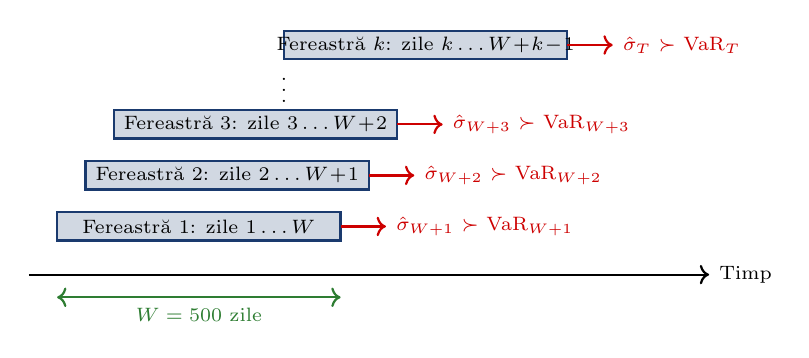
\begin{tikzpicture}[scale=0.72, every node/.style={font=\scriptsize}]
        % Timeline
        \draw[->, thick] (0,0) -- (12,0) node[right] {Timp};

        % Window 1
        \draw[fill=MainBlue!20, draw=MainBlue, thick] (0.5,0.6) rectangle (5.5,1.1);
        \node at (3,0.85) {Fereastră 1: zile $1 \ldots W$};
        \draw[->, thick, IDAred] (5.5,0.85) -- (6.3,0.85) node[right] {$\hat{\sigma}_{W+1}$ $\succ$ VaR$_{W+1}$};

        % Window 2
        \draw[fill=MainBlue!20, draw=MainBlue, thick] (1.0,1.5) rectangle (6.0,2.0);
        \node at (3.5,1.75) {Fereastră 2: zile $2 \ldots W\!+\!1$};
        \draw[->, thick, IDAred] (6.0,1.75) -- (6.8,1.75) node[right] {$\hat{\sigma}_{W+2}$ $\succ$ VaR$_{W+2}$};

        % Window 3
        \draw[fill=MainBlue!20, draw=MainBlue, thick] (1.5,2.4) rectangle (6.5,2.9);
        \node at (4,2.65) {Fereastră 3: zile $3 \ldots W\!+\!2$};
        \draw[->, thick, IDAred] (6.5,2.65) -- (7.3,2.65) node[right] {$\hat{\sigma}_{W+3}$ $\succ$ VaR$_{W+3}$};

        % Dots
        \node at (4.5,3.4) {$\vdots$};

        % Window T
        \draw[fill=MainBlue!20, draw=MainBlue, thick] (4.5,3.8) rectangle (9.5,4.3);
        \node at (7,4.05) {Fereastră $k$: zile $k \ldots W\!+\!k\!-\!1$};
        \draw[->, thick, IDAred] (9.5,4.05) -- (10.3,4.05) node[right] {$\hat{\sigma}_{T}$ $\succ$ VaR$_{T}$};

        % Annotations
        \draw[<->, thick, Forest] (0.5,-0.4) -- (5.5,-0.4) node[midway, below] {$W = 500$ zile};
    \end{tikzpicture}
    \end{center}
    \vspace{-0.2cm}
    {\small
    \begin{block}{Rezultat}
        \begin{itemize}\setlength{\itemsep}{0pt}
            \item Obținem seria $\{\text{VaR}_{\alpha,t}\}_{t=W+1}^{T}$ $\succ$ un prag \textbf{diferit} în fiecare zi
            \item VaR-ul se adaptează la regimul curent: crește în perioadele volatile, scade în cele calme
            \item Comparăm $r_t$ cu $-\text{VaR}_{\alpha,t}$ pentru a identifica încălcările
        \end{itemize}
    \end{block}
    }
\end{frame}

\begin{frame}{Prognoza volatilității cu intervale de încredere}
    \vspace{-0.2cm}
    {\scriptsize
    \begin{cminipage}{0.95\textwidth}
        \vspace{-0.2cm}
        {\footnotesize
        \begin{block}{Interpretare}
            \begin{itemize}\setlength{\itemsep}{0pt}
                \item Prognoza converge către $\bar{\sigma}$
                \item Incertitudinea crește cu orizontul de prognoză
            \end{itemize}
        \end{block}
        }
    \end{cminipage}
    }
    \begin{center}
        \includegraphics[width=0.95\textwidth, height=0.50\textheight, keepaspectratio]{garch_volatility_forecast.pdf}
    \end{center}
    \quantlet{TSA\_ch5\_vol\_ci}{https://github.com/QuantLet/TSA/tree/main/TSA_ch5/TSA_ch5_vol_ci}
\end{frame}

\begin{frame}{Rolling forecast $\succ$ prognoza pas cu pas}
    \vspace{-0.2cm}
    {\scriptsize
    \small
        \begin{block}{Procedura}
        {\footnotesize
            S\&P 500, W=500, GARCH(1,1)-t
            \begin{itemize}\setlength{\itemsep}{1pt}
                \item Re-estimare GARCH pe $[t\!-\!W,\; t\!-\!1]$; prognoză $\hat{\sigma}_{t|t-1}$
                \item Comparație cu vol.\ realizată (std.\ rulantă 20 zile)
            \end{itemize}
        }
        \end{block}
        \vspace{-0.1cm}
        \begin{exampleblock}{Rezultate (2015 zile OOS)}
        {\footnotesize
            \begin{itemize}\setlength{\itemsep}{1pt}
                \item $\rho = 0.938$ $\succ$ urmărire excelentă; MAE $= 0.15\%$, RMSE $= 0.24\%$
                \item COVID-19: sub-predicție temporară, adaptare rapidă
            \end{itemize}
        }
        \end{exampleblock}
    }
\end{frame}

\begin{frame}{Rolling forecast $\succ$ prognoza pas cu pas}
    \begin{center}
        \includegraphics[width=0.95\textwidth, height=0.78\textheight, keepaspectratio]{garch_rolling_forecast.pdf}
    \end{center}
    \quantlet{TSA\_ch5\_rolling\_forecast}{https://github.com/QuantLet/TSA/tree/main/TSA_ch5/TSA_ch5_rolling_forecast}
\end{frame}

%=============================================================================
% SECȚIUNEA 7: IMPLEMENTARE ÎN PYTHON
%=============================================================================
\section{Implementare în Python}

\begin{frame}{VaR backtesting: testul Kupiec}
    \begin{block}{Testul acoperirii necondiționate}
        \begin{itemize}\setlength{\itemsep}{0pt}
            \item Testează dacă rata de încălcare observată este egală cu rata așteptată $p$ (ex.\ 1\% pentru VaR 1\%)
            \item Fie $N$ = numărul de încălcări VaR, $T$ = totalul observațiilor, $\hat{p} = N/T$
            \item \textbf{Statistica Likelihood Ratio:}
            \[
                LR_{uc} = -2\ln\left[\frac{(1-p)^{T-N} p^N}{(1-\hat{p})^{T-N} \hat{p}^N}\right] \sim \chi^2(1)
            \]
        \end{itemize}
    \end{block}

    \vspace{0.2cm}

    \begin{alertblock}{Ipoteze}
        \begin{itemize}\setlength{\itemsep}{0pt}
            \item $H_0$: $\hat{p} = p$ (modelul VaR este corect calibrat)
            \item $H_1$: $\hat{p} \neq p$ (modelul VaR sub- sau supra-estimează riscul)
        \end{itemize}
    \end{alertblock}
\end{frame}

\begin{frame}{VaR backtesting: testul Christoffersen}
    \begin{cminipage}{0.95\textwidth}
        \vspace{-0.3cm}
        \begin{block}{Testul acoperirii condiționate}
            \begin{itemize}\setlength{\itemsep}{0pt}
                \item Testează atât \textbf{acoperirea necondiționată} cât și \textbf{independența} încălcărilor
                \item Încălcările trebuie să fie independente --- fără clusterizare a excepțiilor!
            \end{itemize}
        \end{block}
        \vspace{-0.1cm}
        \begin{block}{Componente ale testului}
            \begin{itemize}\setlength{\itemsep}{0pt}
                \item \textbf{Testul de independență} ($LR_{ind}$): Testează dacă încălcările sunt serial independente
                \item \textbf{Acoperire condiționată}: $LR_{cc} = LR_{uc} + LR_{ind} \sim \chi^2(2)$
            \end{itemize}
        \end{block}
        \vspace{-0.1cm}
        \begin{alertblock}{Interpretare}
            \begin{itemize}\setlength{\itemsep}{0pt}
                \item Respinge $LR_{uc}$: frecvență greșită
                \item Respinge $LR_{ind}$: încălcări clusterizate
                \item Respinge $LR_{cc}$: modelul eșuează
            \end{itemize}
        \end{alertblock}
    \end{cminipage}
\end{frame}

\begin{frame}{Backtesting complet $\succ$ rezultate și decizie}
    \small
    \begin{block}{Aplicare S\&P 500 (T=500, VaR 1\%)}
        \begin{itemize}\setlength{\itemsep}{0pt}
            \item Rolling window: $W = 500$ zile, model EGARCH(1,1)-t
            \item Fereastră de test: $T - W$ zile out-of-sample
            \item Se compară VaR prognozat cu randamentul realizat în fiecare zi
        \end{itemize}
    \end{block}
    \begin{exampleblock}{Output tipic}
        \begin{itemize}\setlength{\itemsep}{0pt}
            \item Număr încălcări vs așteptat $\succ$ zona Basel (verde/galben/roșu)
            \item Kupiec (frecvență): $H_0$: $\hat{p} = \alpha$ $\succ$ p-value $> 0.05$ $\succ$ acceptat
            \item Christoffersen (independență): $H_0$: încălcări i.i.d. $\succ$ p-value $> 0.05$ $\succ$ acceptat
            \item Test combinat: ambele condiții îndeplinite $\succ$ \textcolor{Forest}{\textbf{model validat}}
        \end{itemize}
    \end{exampleblock}
    \quantlet{TSA\_ch5\_backtest\_full}{https://github.com/QuantLet/TSA/tree/main/TSA_ch5/TSA_ch5_backtest_full}
\end{frame}

\begin{frame}{Backtesting-ul Expected Shortfall}
    \begin{cminipage}{0.95\textwidth}
        \scriptsize
        \setlength{\abovedisplayskip}{2pt}\setlength{\belowdisplayskip}{2pt}
        \vspace{-0.3cm}
        \begin{block}{De ce backtesting ES?}
            \begin{itemize}\setlength{\itemsep}{0pt}
                \item VaR măsoară doar \textit{pragul} pierderilor extreme, nu \textit{magnitudinea} lor
                \item ES = pierderea medie \textit{dacă} VaR este depășit $\succ$ mai informativ pentru riscul de coadă
            \end{itemize}
        \end{block}
        \vspace{-0.15cm}
        \begin{defn}[Testul Z Acerbi-Sz\'ekely (2014)]
            \[
                Z_{\text{ES}} = \frac{1}{n_\alpha} \sum_{t: r_t < -\text{VaR}_t} \frac{r_t}{\text{ES}_t} + 1
            \]
            \begin{itemize}\setlength{\itemsep}{0pt}
                \item Sub $H_0$ (model ES corect): $\E[Z_{\text{ES}}] = 0$
                \item Se respinge dacă $Z_{\text{ES}} < z_{\alpha/2}$
            \end{itemize}
        \end{defn}
        \vspace{-0.15cm}
        \begin{alertblock}{Observație}
            \begin{itemize}\setlength{\itemsep}{0pt}
                \item Spre deosebire de backtesting VaR (hit/miss binar), backtesting ES folosește \textit{magnitudinea} pierderilor
                \item Mai puternic dar necesită eșantioane mari ($T > 1000$)
                \item Alternativă: bootstrap McNeil \& Frey (2000)
                \item ES sub Student-$t$: cozi groase $\succ$ ES mai mare decât sub normalitate
            \end{itemize}
        \end{alertblock}
    \end{cminipage}
\end{frame}

\begin{frame}{Basel IV: de la VaR la ES}
    \begin{cminipage}{0.95\textwidth}
        \small
        \begin{block}{Schimbarea reglementară}
            \begin{itemize}\setlength{\itemsep}{0pt}
                \item \textbf{Basel II/III}: Capital bazat pe VaR 99\% (10 zile)
                \item \textbf{Basel IV} (FRTB --- Fundamental Review of the Trading Book, 2023+)
                \item Capital bazat pe \textbf{ES 97.5\%} (10 zile)
                \item Motivație: ES este \textbf{coerent} (subaditivitate), VaR nu este
            \end{itemize}
        \end{block}
        \vspace{-0.1cm}
        \begin{exampleblock}{Echivalență sub normalitate}
            \[
                \text{ES}_{97.5\%}^{\text{Normal}} = \frac{\phi(z_{0.025})}{0.025} \cdot \sigma \approx 2.338\,\sigma \quad \approx \quad \text{VaR}_{99\%}^{\text{Normal}} = 2.326\,\sigma
            \]
            \begin{itemize}\setlength{\itemsep}{0pt}
                \item Sub normalitate, ES 97.5\% $\approx$ VaR 99\%
                \item Sub cozi groase, ES $\gg$ VaR
            \end{itemize}
        \end{exampleblock}
        \vspace{-0.1cm}
        \begin{alertblock}{Implicație practică}
            \begin{itemize}\setlength{\itemsep}{0pt}
                \item Modelele GARCH Student-$t$ devin \textbf{esențiale} pentru estimarea precisă a ES
                \item Băncile trebuie să modeleze \textit{întreaga coadă}, nu doar un singur cuantil
            \end{itemize}
        \end{alertblock}
    \end{cminipage}
\end{frame}

%=============================================================================
% SECȚIUNEA 7b: MODELARE COMBINATĂ ARMA-GARCH
%=============================================================================

\begin{frame}{ARMA-GARCH: modelarea combinată a mediei și varianței}
    \begin{cminipage}{0.95\textwidth}
        \small
        \begin{block}{De ce modelare combinată?}
            \begin{itemize}\setlength{\itemsep}{0pt}
                \item \textbf{Corelație serială} $\succ$ ARMA pentru medie
                \item \textbf{Volatility clustering} $\succ$ GARCH pentru varianță
            \end{itemize}
        \end{block}
        \vspace{-0.1cm}
        \begin{defn}[ARMA(p,q)-GARCH(r,s)]
            \textbf{Ecuația mediei}: $r_t = \mu + \sum_{i=1}^{p} \phi_i (r_{t-i} - \mu) + \sum_{j=1}^{q} \theta_j \varepsilon_{t-j} + \varepsilon_t$

            \textbf{Ecuația varianței}: $\varepsilon_t = \sigma_t z_t$, \quad $\sigma_t^2 = \omega + \sum_{i=1}^{r} \alpha_i \varepsilon_{t-i}^2 + \sum_{j=1}^{s} \beta_j \sigma_{t-j}^2$
        \end{defn}
    \end{cminipage}
\end{frame}

\begin{frame}{ARMA-GARCH: strategie de selecție a modelului}
    \begin{cminipage}{0.95\textwidth}
        \small
        \begin{block}{Abordare pas cu pas}
            \begin{enumerate}\setlength{\itemsep}{0pt}
                \item \textbf{Identifică modelul pentru medie}: Verifică ACF/PACF al randamentelor
                \item \textbf{Testează efectele ARCH}: Aplică testul ARCH-LM pe reziduuri
                \item \textbf{Specifică modelul pentru varianță}: De obicei GARCH(1,1) este suficient
                \item \textbf{Estimare combinată}: Estimează ambele ecuații prin MLE
                \item \textbf{Diagnostic}: Reziduurile standardizate trebuie să fie i.i.d.
            \end{enumerate}
        \end{block}

        \vspace{0.2cm}

        \begin{alertblock}{Specificații comune}
            \begin{itemize}\setlength{\itemsep}{0pt}
                \item \textbf{Randamente acțiuni}: AR(1)-GARCH(1,1) sau ARMA(1,1)-GARCH(1,1)
                \item \textbf{Cursuri de schimb}: Adesea doar GARCH(1,1) (fără dinamică în medie)
                \item \textbf{Rate ale dobânzii}: AR(1)-EGARCH(1,1) pentru efecte de levier
            \end{itemize}
        \end{alertblock}
    \end{cminipage}
\end{frame}

\begin{frame}[fragile]{Python: Estimarea GARCH cu \texttt{arch}}
    \begin{cminipage}{0.95\textwidth}
        \vspace{-2mm}
        \begin{block}{Pași principali}
    \begin{lstlisting}
from arch import arch_model
import numpy as np
from scipy.stats import norm

# Fit GARCH(1,1) with Student-t innovations
model = arch_model(returns, vol='Garch', p=1, q=1,
                   dist='StudentsT', mean='AR', lags=1)
result = model.fit(disp='off')
print(result.summary())

# Forecast 20-step ahead volatility
forecast = result.forecast(horizon=20)
sigma_forecast = np.sqrt(forecast.variance.iloc[-1])

# Compute 1-day VaR (1%) from conditional distribution
sigma_1 = sigma_forecast.iloc[0]
VaR_1pct = norm.ppf(0.01) * sigma_1  # Normal approx
    \end{lstlisting}
        \end{block}
        \vspace{-2mm}
        {\scriptsize \textbf{Notă}: Pentru VaR Student-$t$, înlocuiți \texttt{norm.ppf} cu \texttt{scipy.stats.t.ppf(0.01, df=nu)} scalat cu $\sqrt{(\nu-2)/\nu}$.}
    \end{cminipage}
\end{frame}

%=============================================================================
% SECȚIUNEA 8: STUDIU DE CAZ --- S&P 500
%=============================================================================
\section{Studiu de Caz: S\&P 500}

\begin{frame}{Pasul 1: Datele $\succ$ randamente zilnice S\&P 500}
    \vspace{-0.2cm}
    {\scriptsize
    {\small
        \begin{block}{Descrierea datelor}
            \begin{itemize}\setlength{\itemsep}{0pt}
                \item \textbf{Sursă}: Yahoo Finance, S\&P 500, date zilnice 2000--2024 ($T > 6000$)
                \item \textbf{Randamente}: $r_t = \ln(P_t/P_{t-1}) \times 100$
            \end{itemize}
        \end{block}
        \vspace{-0.2cm}
        \begin{exampleblock}{Statistici descriptive}
            \vspace{-0.1cm}
            \begin{center}
            {\footnotesize
            \begin{tabular}{cccccc}
                \toprule
                Medie & Std. Dev. & Skewness & Kurtosis & Min & Max \\
                \midrule
                0.034\% & 1.21\% & $-0.29$ & 13.8 & $-12.8\%$ & $+11.0\%$ \\
                \bottomrule
            \end{tabular}
            }
            \end{center}
            \vspace{-0.1cm}
            \begin{itemize}\setlength{\itemsep}{0pt}
                \item Cozi groase (kurtosis $\gg 3$) și asimetrie negativă $\succ$ efecte ARCH
            \end{itemize}
        \end{exampleblock}
        }
    }
\end{frame}

\begin{frame}{Pasul 1: Datele $\succ$ randamente zilnice S\&P 500}
    \begin{center}
        \includegraphics[width=0.95\textwidth, height=0.78\textheight, keepaspectratio]{garch_sp500_returns.pdf}
    \end{center}
    \quantlet{TSA\_ch5\_sp500}{https://github.com/QuantLet/TSA/tree/main/TSA_ch5/TSA_ch5_sp500}
\end{frame}

\begin{frame}{Pasul 2: Testarea efectelor ARCH}
    \small
    \begin{block}{Cod Python $\succ$ ARCH-LM și Ljung-Box pe $r_t^2$}
        \begin{itemize}\setlength{\itemsep}{0pt}
            \item Testăm prezența efectelor ARCH în reziduurile modelului pentru medie
        \end{itemize}
    \end{block}
    \begin{exampleblock}{Rezultate}
        {\small
        \begin{tabular}{lcc}
            \toprule
            \textbf{Test} & \textbf{Statistică} & \textbf{p-value} \\
            \midrule
            ARCH-LM (10 lags) & 892.4 & $< 0.0001$ \\
            Ljung-Box $r_t^2$ (lag 20) & 4217.6 & $< 0.0001$ \\
            \bottomrule
        \end{tabular}
        }
        \begin{itemize}\setlength{\itemsep}{0pt}
            \item \textbf{Concluzie}: Efecte ARCH puternice $\succ$ heteroscedasticitate semnificativă
        \end{itemize}
    \end{exampleblock}
\end{frame}

\begin{frame}{Pasul 3: Parametri estimați $\succ$ comparație}
    \vspace{-0.2cm}
    {\scriptsize
    {\scriptsize
        \begin{block}{Tabel parametri estimați}
            \begin{center}
            \begin{tabular}{lccccccc}
                \toprule
                \textbf{Model} & $\omega$ & $\alpha$ & $\beta$ & $\gamma$ & $\alpha\!+\!\beta$ & $\nu$ & \textbf{HL} \\
                \midrule
                GARCH-N & 0.011 & 0.088 & 0.901 & --- & 0.989 & --- & 60 zile \\
                GARCH-t & 0.011 & 0.088 & 0.900 & --- & 0.989 & 6.42 & 60 zile \\
                EGARCH-t & 0.003 & 0.103 & 0.987 & $-$0.120 & --- & 6.38 & 53 zile \\
                GJR-t & 0.010 & 0.022 & 0.906 & 0.126 & 0.991 & 6.51 & 78 zile \\
                \bottomrule
            \end{tabular}
            \end{center}
        \end{block}
        \vspace{-0.1cm}
        \begin{alertblock}{Interpretare}
            \begin{itemize}\setlength{\itemsep}{0pt}
                \item EGARCH $\gamma = -0.12$ \textbf{semnificativ} $\succ$ \textbf{leverage effect confirmat}
                \item GJR: $\alpha_{\text{neg}} = \alpha + \gamma = 0.148$ vs $\alpha_{\text{poz}} = 0.022$ $\succ$ asimetrie puternică
            \end{itemize}
        \end{alertblock}
        }
    }
\end{frame}

\begin{frame}{Pasul 3: Volatilitatea condiționată estimată $\succ$ S\&P 500}
    \begin{center}
        \includegraphics[width=0.95\textwidth, height=0.78\textheight, keepaspectratio]{garch_sp500_volatility.pdf}
    \end{center}
    \quantlet{TSA\_ch5\_sp500\_garch}{https://github.com/QuantLet/TSA/tree/main/TSA_ch5/TSA_ch5_sp500_garch}
\end{frame}

\begin{frame}{Pasul 5: Leverage effect $\succ$ vizualizare}
    \vspace{-0.2cm}
    {\footnotesize
        \begin{block}{GARCH vs EGARCH $\succ$ diferențe de volatilitate}
            \begin{itemize}\setlength{\itemsep}{0pt}
                \item EGARCH produce volatilitate \textbf{mai mare} după șocuri negative (2008, 2020)
                \item GARCH simetric \textbf{subestimează} riscul în perioadele de criză
                \item Diferența: până la 2--3 puncte procentuale în volatilitate zilnică
            \end{itemize}
        \end{block}
    }
    \begin{center}
        \includegraphics[width=0.95\textwidth, height=0.50\textheight, keepaspectratio]{garch_sp500_comparison.pdf}
    \end{center}
    \quantlet{TSA\_ch5\_sp500\_comp}{https://github.com/QuantLet/TSA/tree/main/TSA_ch5/TSA_ch5_sp500_comp}
\end{frame}

\begin{frame}{Pasul 4: Selecția modelului $\succ$ AIC/BIC}
    \begin{cminipage}{0.95\textwidth}
        \begin{block}{Criterii informaționale}
            \begin{center}
            {\small
            \begin{tabular}{lcccl}
                \toprule
                \textbf{Model} & \textbf{Log-Lik} & \textbf{AIC} & \textbf{BIC} & \textbf{Rang} \\
                \midrule
                GARCH(1,1)-N & $-$8042.3 & 16090.6 & 16111.0 & 4 \\
                GARCH(1,1)-t & $-$7981.5 & 15971.0 & 15997.8 & 3 \\
                EGARCH(1,1)-t & $-$7964.2 & \textbf{15938.4} & \textbf{15971.6} & \textbf{1} \\
                GJR-GARCH(1,1)-t & $-$7968.1 & 15946.2 & 15979.4 & 2 \\
                \bottomrule
            \end{tabular}
            }
            \end{center}
        \end{block}
        \begin{exampleblock}{Decizia}
            \begin{itemize}\setlength{\itemsep}{0pt}
                \item \textbf{EGARCH(1,1)-t câștigă}: cel mai mic AIC \textbf{și} BIC
                \item Student-t superior normalei ($\Delta$AIC $\approx 120$) $\succ$ cozi groase contează!
                \item Leverage effect justifică modele asimetrice ($\Delta$AIC $\approx 33$ față de GARCH-t)
            \end{itemize}
        \end{exampleblock}
    \end{cminipage}
\end{frame}

\begin{frame}{Pasul 5: Diagnostice $\succ$ EGARCH(1,1)-t}
    \begin{cminipage}{0.95\textwidth}
        {\small
        \begin{block}{Verificări pe reziduuri standardizate $z_t = \varepsilon_t / \hat{\sigma}_t$}
            \begin{itemize}\setlength{\itemsep}{0pt}
                \item \textbf{Ljung-Box} pe $z_t$: p-value $= 0.38$ $\succ$ fără autocorelație reziduală
                \item \textbf{Ljung-Box} pe $z_t^2$: p-value $= 0.52$ $\succ$ \textbf{efecte ARCH eliminate}
                \item \textbf{Q-Q plot}: punctele urmează dreapta teoretică Student-t
                \item \textbf{Concluzie}: modelul EGARCH(1,1)-t captează adecvat dinamica volatilității
            \end{itemize}
        \end{block}
        }
    \end{cminipage}
\end{frame}

\begin{frame}{Pasul 5: Diagnostice $\succ$ EGARCH(1,1)-t}
    \begin{center}
        \includegraphics[width=0.95\textwidth, height=0.78\textheight, keepaspectratio]{garch_diagnostics.pdf}
    \end{center}
    \quantlet{TSA\_ch5\_sp500\_diag}{https://github.com/QuantLet/TSA/tree/main/TSA_ch5/TSA_ch5_sp500_diag}
\end{frame}

\begin{frame}{Pasul 6: Backtesting rolling VaR $\succ$ S\&P 500}
    \vspace{-0.2cm}
    {\scriptsize
    {\small
        \begin{exampleblock}{Rezultate Kupiec + Christoffersen (2015 zile out-of-sample)}
            \vspace{-0.1cm}
            \begin{center}
            {\footnotesize
            \begin{tabular}{lccl}
                \toprule
                \textbf{Test} & \textbf{Statistică} & \textbf{p-value} & \textbf{Decizia} \\
                \midrule
                Încălcări & 27/2015 ($\hat{p}=1.34\%$) & --- & Zona \textcolor{Forest}{\textbf{verde}} \\
                Kupiec (uc) & 2.13 & 0.145 & \textcolor{Forest}{Acceptat} \\
                Christoffersen (ind) & 0.79 & 0.375 & \textcolor{Forest}{Acceptat} \\
                Combinat (cc) & 2.91 & 0.233 & \textcolor{Forest}{Acceptat} \\
                \bottomrule
            \end{tabular}
            }
            \end{center}
        \end{exampleblock}
        }
    }
\end{frame}

\begin{frame}{Pasul 6: Rolling VaR $\succ$ S\&P 500}
    \begin{center}
        \includegraphics[width=0.95\textwidth, height=0.78\textheight, keepaspectratio]{garch_sp500_rolling_var.pdf}
    \end{center}
    \quantlet{TSA\_ch5\_sp500\_var}{https://github.com/QuantLet/TSA/tree/main/TSA_ch5/TSA_ch5_sp500_var}
\end{frame}

\begin{frame}{Pasul 7: Concluzii $\succ$ studiu S\&P 500}
    \begin{cminipage}{0.95\textwidth}
        \begin{block}{Rezumatul metodologiei pas cu pas}
            \begin{enumerate}\setlength{\itemsep}{2pt}
                \item \textbf{Date}: randamente log, statistici descriptive $\succ$ cozi groase, asimetrie
                \item \textbf{Test ARCH}: ARCH-LM + Ljung-Box pe $r_t^2$ $\succ$ efecte ARCH semnificative
                \item \textbf{Estimare}: 4 modele candidate (simetric/asimetric $\times$ Normal/Student-t)
                \item \textbf{Selecție}: AIC/BIC $\succ$ \textbf{EGARCH(1,1)-t} câștigător
                \item \textbf{Diagnostice}: reziduuri standardizate $\succ$ model adecvat
                \item \textbf{VaR}: rolling window + backtesting Kupiec/Christoffersen $\succ$ model \textbf{validat}
            \end{enumerate}
        \end{block}
        \vspace{0.1cm}
        \begin{alertblock}{Concluzii}
            \begin{itemize}\setlength{\itemsep}{0pt}
                \item Distribuția Student-t este \textbf{esențială} pentru date financiare
                \item Leverage effect: modelele asimetrice \textbf{obligatorii} pentru acțiuni
                \item Backtesting sistematic: nu doar „arată bine'', ci \textbf{testat statistic}
            \end{itemize}
        \end{alertblock}
    \end{cminipage}
\end{frame}

%=============================================================================
% SECȚIUNEA 9: STUDIU DE CAZ --- Bitcoin
%=============================================================================
\section{Studiu de Caz: Bitcoin}

\begin{frame}{Pasul 1: Datele $\succ$ randamente zilnice Bitcoin}
    \vspace{-0.2cm}
    {\scriptsize
        \begin{block}{Descrierea datelor}
            \begin{itemize}\setlength{\itemsep}{0pt}
                \item \textbf{Sursă}: Yahoo Finance (BTC-USD), date zilnice 2018--2024
                \item Randamente log: media $\approx 0.05\%$, volatilitate $\approx 3.5\%$
            \end{itemize}
        \end{block}
        \vspace{-0.2cm}
        \begin{exampleblock}{Statistici descriptive}
            \vspace{-0.1cm}
            \begin{center}
            {\footnotesize
            \begin{tabular}{cccccc}
                \toprule
                Medie & Std. Dev. & Skewness & Kurtosis & Min & Max \\
                \midrule
                0.05\% & 3.48\% & $-0.72$ & 12.1 & $-46.5\%$ & $+22.5\%$ \\
                \bottomrule
            \end{tabular}
            }
            \end{center}
            \vspace{-0.15cm}
            \begin{itemize}\setlength{\itemsep}{0pt}
                \item Volatilitate $\sim$3$\times$ mai mare decât S\&P 500
                \item Kurtosis extremă $\succ$ riscul de pierderi mari
            \end{itemize}
        \end{exampleblock}
        }
\end{frame}

\begin{frame}{Pasul 1: Datele $\succ$ randamente zilnice Bitcoin}
    \begin{center}
        \includegraphics[width=0.95\textwidth, height=0.78\textheight, keepaspectratio]{btc_returns.pdf}
    \end{center}
    \quantlet{TSA\_ch5\_btc}{https://github.com/QuantLet/TSA/tree/main/TSA_ch5/TSA_ch5_btc}
\end{frame}

\begin{frame}{Pasul 2: Testarea efectelor ARCH $\succ$ Bitcoin}
    \vspace{-0.2cm}
    {\scriptsize
    }
    \begin{center}
        \includegraphics[width=0.95\textwidth, height=0.50\textheight, keepaspectratio]{btc_squared_returns.pdf}
    \end{center}
    \quantlet{TSA\_ch5\_btc\_arch}{https://github.com/QuantLet/TSA/tree/main/TSA_ch5/TSA_ch5_btc_arch}
\end{frame}

\begin{frame}{Pasul 5: Volatilitatea condiționată $\succ$ Bitcoin}
    \vspace{-0.2cm}
    {\footnotesize
        \begin{block}{Diagnostice GJR-GARCH(1,1)-t}
            \begin{itemize}\setlength{\itemsep}{0pt}
                \item Ljung-Box pe $z_t^2$: p-value $= 0.41$ $\succ$ \textbf{efecte ARCH eliminate}
                \item Vârfuri volatilitate: martie 2020 (COVID), mai 2022 (Terra/Luna)
                \item Volatilitate zilnică: de la 1\% (perioadele calme) la $>$15\% (crize)
            \end{itemize}
        \end{block}
    }
    \begin{center}
        \includegraphics[width=0.95\textwidth, height=0.50\textheight, keepaspectratio]{ch10_bitcoin_garch.pdf}
    \end{center}
    \quantlet{TSA\_ch5\_btc\_garch}{https://github.com/QuantLet/TSA/tree/main/TSA_ch5/TSA_ch5_btc_garch}
\end{frame}

\begin{frame}{Pasul 3--4: Estimare și selecție modele $\succ$ Bitcoin}
    \begin{cminipage}{0.95\textwidth}
        \begin{block}{Parametri estimați}
            \begin{center}
            {\small
            \begin{tabular}{lccccccc}
                \toprule
                \textbf{Model} & $\omega$ & $\alpha$ & $\beta$ & $\gamma$ & $\alpha\!+\!\beta$ & $\nu$ & \textbf{AIC} \\
                \midrule
                GARCH-t & 0.42 & 0.131 & 0.848 & --- & 0.979 & 4.82 & 9284 \\
                EGARCH-t & 0.08 & 0.184 & 0.976 & $-$0.061 & --- & 4.79 & 9276 \\
                GJR-t & 0.40 & 0.088 & 0.854 & 0.078 & 0.976 & 4.85 & \textbf{9271} \\
                \bottomrule
            \end{tabular}
            }
            \end{center}
        \end{block}
        \begin{block}{Interpretare}
            \begin{itemize}\setlength{\itemsep}{0pt}
                \item \textbf{GJR-GARCH-t câștigă} (cel mai mic AIC)
                \item $\nu \approx 4.8$: cozi \textbf{mult mai groase} decât S\&P 500 ($\nu = 6.4$)
                \item $\alpha = 0.131$ (BTC) vs $0.088$ (S\&P) $\succ$ Bitcoin reacționează mai rapid la informații noi
                \item Leverage effect mai slab decât la acțiuni ($\gamma_{\text{BTC}} = 0.078$ vs $0.126$)
            \end{itemize}
        \end{block}
    \end{cminipage}
\end{frame}

\begin{frame}{Pasul 6: Backtesting rolling VaR $\succ$ Bitcoin}
    \vspace{-0.2cm}
    {\scriptsize
    {\scriptsize
        \begin{block}{Teste statistice (2421 zile out-of-sample)}
            \vspace{-0.15cm}
            \begin{center}
            \begin{tabular}{lccl}
                \toprule
                \textbf{Test} & \textbf{Statistică} & \textbf{p-value} & \textbf{Decizia} \\
                \midrule
                Încălcări & 28/2421 ($\hat{p}=1.16\%$) & --- & Zona \textcolor{Forest}{\textbf{verde}} \\
                Kupiec (uc) & 0.57 & 0.450 & \textcolor{Forest}{Acceptat} \\
                Christoffersen (ind) & 0.94 & 0.333 & \textcolor{Forest}{Acceptat} \\
                Combinat (cc) & 1.51 & 0.471 & \textcolor{Forest}{Acceptat} \\
                \bottomrule
            \end{tabular}
            \end{center}
            \vspace{-0.15cm}
        \end{block}
        \vspace{-0.15cm}
        \begin{alertblock}{Interpretare}
            \begin{itemize}\setlength{\itemsep}{0pt}
                \item Volatilitatea variază de la 3\% la 38\% $\succ$ rolling window \textbf{esențial}
                \item Toate testele \textbf{acceptate}: model valid pentru managementul riscului
            \end{itemize}
        \end{alertblock}
        }
    }
\end{frame}

\begin{frame}{Pasul 6: Rolling VaR $\succ$ Bitcoin}
    \begin{center}
        \includegraphics[width=0.95\textwidth, height=0.78\textheight, keepaspectratio]{garch_btc_rolling_var.pdf}
    \end{center}
    \quantlet{TSA\_ch5\_btc\_var}{https://github.com/QuantLet/TSA/tree/main/TSA_ch5/TSA_ch5_btc_var}
\end{frame}

\begin{frame}{Pasul 6: VaR rolling window $\succ$ Bitcoin}
    \small
    \begin{block}{Rolling window GJR-GARCH-t (W=500 zile, VaR 1\%)}
        \begin{itemize}\setlength{\itemsep}{0pt}
            \item Estimare rolling pe fereastră de 500 zile cu prognoză VaR zilnică
        \end{itemize}
    \end{block}
    {\small
    \begin{exampleblock}{Caracteristici VaR rolling Bitcoin (2018--2024)}
        \begin{itemize}\setlength{\itemsep}{0pt}
            \item VaR mediu: 9.34\% ($\approx$ EUR 93.400 / 1M EUR)
            \item VaR maxim: 37.54\% $\succ$ crash COVID martie 2020
            \item VaR minim: 2.90\% $\succ$ perioadă calmă
            \item Bitcoin: VaR rolling $\sim$4$\times$ mai mare decât S\&P 500 la aceeași expunere
        \end{itemize}
    \end{exampleblock}
    }
\end{frame}

\begin{frame}{Comparație finală: S\&P 500 vs Bitcoin}
    \begin{cminipage}{0.95\textwidth}
        \vspace{-0.3cm}
        {\small
        \begin{block}{Rezumat comparativ}
            \vspace{-0.1cm}
            \begin{center}
            {\footnotesize
            \begin{tabular}{lcc}
                \toprule
                & \textbf{S\&P 500} & \textbf{Bitcoin} \\
                \midrule
                Volatilitate medie & 1.2\% & 3.5\% \\
                Kurtosis & 13.8 & 12.1 \\
                Student-t $\nu$ & 6.42 & 4.82 \\
                Cel mai bun model & EGARCH(1,1)-t & GJR-GARCH(1,1)-t \\
                Leverage effect & Puternic ($\gamma = -0.12$) & Moderat ($\gamma = 0.078$) \\
                Half-life & $\sim$60 zile & $\sim$42 zile \\
                Rolling VaR 1\% mediu & \textcolor{Forest}{\textbf{2.53\%}} & \textcolor{Forest}{\textbf{9.34\%}} \\
                Rolling VaR 1\% maxim & \textcolor{Crimson}{\textbf{22.02\%}} (COVID) & \textcolor{Crimson}{\textbf{37.54\%}} (COVID) \\
                Rolling ES 1\% mediu & \textcolor{Forest}{\textbf{3.42\%}} & \textcolor{Forest}{\textbf{12.87\%}} \\
                Kupiec & \textcolor{Forest}{\textbf{Acceptat}} (p=0.145) & \textcolor{Forest}{\textbf{Acceptat}} (p=0.450) \\
                Christoffersen (ind) & \textcolor{Forest}{\textbf{Acceptat}} (p=0.375) & \textcolor{Forest}{\textbf{Acceptat}} (p=0.333) \\
                \bottomrule
            \end{tabular}
            }
            \end{center}
        \end{block}
        \vspace{-0.1cm}
        \begin{alertblock}{Concluzie generală}
            \begin{itemize}\setlength{\itemsep}{0pt}
                \item Re-estimare GARCH la fiecare pas: Kupiec + Christoffersen \textbf{acceptate}
                \item Rolling window VaR: \textbf{obligatoriu} $\succ$ VaR static complet inadecvat
                \item Student-t + model asimetric: \textbf{esențiale} pentru ambele piețe
            \end{itemize}
        \end{alertblock}
        }
    \end{cminipage}
\end{frame}

%=============================================================================
% FORMULE PRINCIPALE
%=============================================================================
\begin{frame}{Formule principale}
    \begin{cminipage}{0.95\textwidth}
        \small
        \begin{block}{Modele de volatilitate}
            \begin{itemize}\setlength{\itemsep}{0pt}
                \item \textbf{ARCH(q):} $\sigma_t^2 = \omega + \sum_{i=1}^{q} \alpha_i \varepsilon_{t-i}^2$
                \item \textbf{GARCH(1,1):} $\sigma_t^2 = \omega + \alpha \varepsilon_{t-1}^2 + \beta \sigma_{t-1}^2$
                \item \textbf{EGARCH:} $\ln(\sigma_t^2) = \omega + \alpha(|z_{t-1}| - \E[|z|]) + \gamma z_{t-1} + \beta \ln(\sigma_{t-1}^2)$
                \item \textbf{GJR-GARCH:} $\sigma_t^2 = \omega + \alpha \varepsilon_{t-1}^2 + \gamma \varepsilon_{t-1}^2 I_{t-1} + \beta \sigma_{t-1}^2$
            \end{itemize}
        \end{block}

        \begin{block}{Proprietăți și măsuri}
            \begin{itemize}\setlength{\itemsep}{0pt}
                \item \textbf{Var. necond.:} $\bar{\sigma}^2 = \frac{\omega}{1-\alpha-\beta}$ \quad \textbf{Half-life:} $HL = \frac{\ln(0.5)}{\ln(\alpha+\beta)}$
                \item \textbf{VaR:} $\text{VaR}_\alpha = z_\alpha \cdot \sigma_{T+1}$ \quad \textbf{Staționaritate:} $\alpha + \beta < 1$
                \item \textbf{ARCH-LM:} $LM = T \cdot R^2 \sim \chi^2(q)$
            \end{itemize}
        \end{block}
    \end{cminipage}
\end{frame}

%=============================================================================
\section{Utilizare IA}
%=============================================================================

\begin{frame}{Exercițiu AI: Gândire critică}
    \begin{cminipage}{0.95\textwidth}
        \vspace{-3mm}
        \begin{block}{\footnotesize Prompt de testat în ChatGPT / Claude / Copilot}
            {\footnotesize
            ``Folosind yfinance, descarcă prețurile zilnice de închidere S\&P 500 (\^{}GSPC) din 2018-01-01 până în 2024-12-31 (aprox.\ 1.750 observații). Calculează randamentele logaritmice zilnice. Testează efectele ARCH, ajustează un model GARCH(1,1) și prognozează volatilitatea pe următoarele 20 de zile de tranzacționare. Vreau cod Python complet.''
            }
        \end{block}
        \vspace{-2mm}
        {\footnotesize
        \textbf{Exercițiu}:
        \begin{enumerate}\setlength{\itemsep}{0pt}
            \item Rulați prompt-ul într-un LLM la alegere și analizați critic răspunsul
            \item Calculează randamentele logaritmice corect? Elimină media înainte de GARCH?
            \item Cum testează efectele ARCH? Folosește testul LM al lui Engle?
            \item Separă ecuația mediei de ecuația varianței?
            \item Discută efectele asimetrice (GJR-GARCH, EGARCH)?
        \end{enumerate}
        }
    \end{cminipage}
\end{frame}

\begin{frame}{Exercițiu AI: Gândire critică (cont.)}
    \begin{cminipage}{0.95\textwidth}
        {\footnotesize
        \textbf{Exercițiu (continuare)}:
        \begin{enumerate}\setlength{\itemsep}{0pt}
            \setcounter{enumi}{5}
            \item Estimările VaR sunt calculate din distribuția condițională?
            \item Identificați cel puțin \textbf{două erori factuale} sau presupuneri discutabile din output-ul LLM
            \item Verifică codul constrângerea de staționaritate $\alpha + \beta < 1$? Dacă nu, adăugați-o
            \item Comparați estimarea VaR a LLM-ului cu rezultatele din acest capitol. Sunt consistente?
        \end{enumerate}
        }
        \vspace{-2mm}
        \begin{alertblock}{}
            {\footnotesize \textbf{Atenție}: Codul generat de AI poate rula fără erori și arăta profesional. \textit{Asta nu înseamnă că e corect.}}
        \end{alertblock}
    \end{cminipage}
\end{frame}

%=============================================================================
% REZUMAT
%=============================================================================
\section{Rezumat}

\begin{frame}{Rezumat $\succ$ capitolul 5: Modele de volatilitate}
    \small
    \vspace{-0.2cm}
    \begin{cminipage}{0.95\textwidth}
        \begin{block}{Concepte fundamentale}
            \begin{itemize}\setlength{\itemsep}{0pt}
                \item \textbf{ARCH(q)}: varianța condiționată depinde de pătratele erorilor trecute (Nobel 2003)
                \item \textbf{GARCH(p,q)}: adaugă lag-uri ale varianței pentru persistență (GARCH(1,1) în 90\% din cazuri)
                \item \textbf{EGARCH}: permite leverage effect, fără restricții de pozitivitate
                \item \textbf{GJR-GARCH/TGARCH}: captură asimetria cu variabile indicador
            \end{itemize}
        \end{block}
        \vspace{-0.2cm}
        \begin{block}{Aplicații}
            \begin{itemize}\setlength{\itemsep}{0pt}
                \item Măsurarea și prognoza riscului (VaR, ES)
                \item Prețul derivatelor, hedging dinamic, managementul portofoliului
            \end{itemize}
        \end{block}
        \vspace{-0.2cm}
        \begin{alertblock}{Sfat practic}
            \begin{itemize}\setlength{\itemsep}{0pt}
                \item Începe cu GARCH(1,1), verifică leverage effect, alege distribuția care minimizează AIC/BIC!
                    \begin{itemize}\setlength{\itemsep}{0pt}
                        \item Student-t adesea superior distribuției normale
                    \end{itemize}
            \end{itemize}
        \end{alertblock}
    \end{cminipage}
\end{frame}

%=============================================================================
% QUIZ
%=============================================================================
\section{Quiz}

\begin{frame}{Întrebarea 1}
    \begin{cminipage}{0.95\textwidth}
        \begin{alertblock}{Întrebare}
            \begin{itemize}\setlength{\itemsep}{0pt}
                \item Ce descrie cel mai bine fenomenul de \textit{volatility clustering} în seriile financiare?
            \end{itemize}
        \end{alertblock}

        \vspace{0.3cm}

        \begin{block}{Variante de răspuns}

            \textcolor{MainBlue}{\textbf{(A)}} Randamentele financiare sunt distribuite normal și independente\\[3pt]

            \textcolor{MainBlue}{\textbf{(B)}} Perioadele de volatilitate ridicată sunt urmate de perioade de volatilitate ridicată, și invers\\[3pt]

            \textcolor{MainBlue}{\textbf{(C)}} Volatilitatea este constantă în timp (homoscedasticitate)\\[3pt]

            \textcolor{MainBlue}{\textbf{(D)}} Corelația dintre randamente este întotdeauna pozitivă

        \end{block}
    \end{cminipage}
\end{frame}

\begin{frame}{Întrebarea 1: Răspuns}
    \begin{cminipage}{0.95\textwidth}
        \vspace{-0.2cm}
        \begin{center}
            \includegraphics[width=0.98\textwidth, height=0.58\textheight, keepaspectratio]{garch_quiz1_volatility_clustering.pdf}
        \end{center}
        \vspace{-3mm}
        {\small
        \begin{exampleblock}{Răspuns: (B)}
            \begin{itemize}\setlength{\itemsep}{0pt}
                \item Volatility clustering este un fapt stilizat fundamental. Implică faptul că varianța condiționată este \textbf{predictibilă}, motivând modelele ARCH/GARCH.
            \end{itemize}
        \end{exampleblock}
        }
        \hfill\quantlet{TSA\_ch5\_quiz1\_volatility\_clustering}{https://github.com/QuantLet/TSA/tree/main/TSA_ch5/TSA_ch5_quiz1_volatility_clustering}
    \end{cminipage}
\end{frame}

\begin{frame}{Întrebarea 2}
    \begin{cminipage}{0.95\textwidth}
        \begin{alertblock}{Întrebare}
            \begin{itemize}\setlength{\itemsep}{0pt}
                \item Care este diferența principală dintre un model ARCH(q) și un model GARCH(p,q)?
            \end{itemize}
        \end{alertblock}

        \vspace{0.3cm}

        \begin{block}{Variante de răspuns}

            \textcolor{MainBlue}{\textbf{(A)}} GARCH modelează media condiționată, ARCH modelează varianța\\[3pt]

            \textcolor{MainBlue}{\textbf{(B)}} ARCH include lag-uri ale varianței condiționate, GARCH nu\\[3pt]

            \textcolor{MainBlue}{\textbf{(C)}} GARCH adaugă lag-uri ale varianței condiționate ($\sigma_{t-j}^2$) pe lângă pătratele erorilor\\[3pt]

            \textcolor{MainBlue}{\textbf{(D)}} ARCH este mai parcimonios decât GARCH

        \end{block}
    \end{cminipage}
\end{frame}

\begin{frame}{Întrebarea 2: Răspuns}
    \begin{cminipage}{0.95\textwidth}
        \vspace{-0.2cm}
        \begin{center}
            \includegraphics[width=0.98\textwidth, height=0.58\textheight, keepaspectratio]{garch_quiz2_arch_vs_garch.pdf}
        \end{center}
        \vspace{-3mm}
        {\small
        \begin{exampleblock}{Răspuns: (C)}
            \begin{itemize}\setlength{\itemsep}{0pt}
                \item GARCH(1,1) captează aceeași persistență ca ARCH(q) cu doar 2 parametri în loc de $q$. În practică, GARCH(1,1) este suficient în 90\% din cazuri.
            \end{itemize}
        \end{exampleblock}
        }
        \hfill\quantlet{TSA\_ch5\_quiz2\_arch\_vs\_garch}{https://github.com/QuantLet/TSA/tree/main/TSA_ch5/TSA_ch5_quiz2_arch_vs_garch}
    \end{cminipage}
\end{frame}

\begin{frame}{Întrebarea 3}
    \begin{cminipage}{0.95\textwidth}
        \begin{alertblock}{Întrebare}
            \begin{itemize}\setlength{\itemsep}{0pt}
                \item Ce este \textit{leverage effect} și ce modele GARCH îl captează?
            \end{itemize}
        \end{alertblock}

        \vspace{0.3cm}

        \begin{block}{Variante de răspuns}

            \textcolor{MainBlue}{\textbf{(A)}} Șocurile pozitive cresc volatilitatea mai mult; captat de GARCH standard\\[3pt]

            \textcolor{MainBlue}{\textbf{(B)}} Șocurile negative cresc volatilitatea mai mult; captat de EGARCH și GJR-GARCH\\[3pt]

            \textcolor{MainBlue}{\textbf{(C)}} Volatilitatea este simetrică; captat de toate modelele GARCH\\[3pt]

            \textcolor{MainBlue}{\textbf{(D)}} Efectul de levier financiar asupra prețului acțiunilor; captat de IGARCH

        \end{block}
    \end{cminipage}
\end{frame}

\begin{frame}{Întrebarea 3: Răspuns}
    \begin{cminipage}{0.95\textwidth}
        \vspace{-0.2cm}
        \begin{center}
            \includegraphics[width=0.98\textwidth, height=0.58\textheight, keepaspectratio]{garch_quiz3_leverage_effect.pdf}
        \end{center}
        \vspace{-3mm}
        {\small
        \begin{exampleblock}{Răspuns: (B)}
            \begin{itemize}\setlength{\itemsep}{0pt}
                \item Scăderile de preț cresc volatilitatea \textbf{mai mult} decât creșterile de aceeași magnitudine. GARCH standard folosește $\varepsilon_{t-1}^2$, pierzând informația de semn.
            \end{itemize}
        \end{exampleblock}
        }
        \hfill\quantlet{TSA\_ch5\_quiz3\_leverage\_effect}{https://github.com/QuantLet/TSA/tree/main/TSA_ch5/TSA_ch5_quiz3_leverage_effect}
    \end{cminipage}
\end{frame}

\begin{frame}{Întrebarea 4}
    \begin{cminipage}{0.95\textwidth}
        \begin{alertblock}{Întrebare}
            \begin{itemize}\setlength{\itemsep}{0pt}
                \item Care este condiția de staționaritate pentru un model GARCH(1,1)?
            \end{itemize}
        \end{alertblock}

        \vspace{0.3cm}

        \begin{block}{Variante de răspuns}

            \textcolor{MainBlue}{\textbf{(A)}} $\alpha + \beta = 1$\\[3pt]

            \textcolor{MainBlue}{\textbf{(B)}} $\alpha > 0$ și $\beta > 0$\\[3pt]

            \textcolor{MainBlue}{\textbf{(C)}} $\alpha + \beta < 1$, cu $\omega > 0$, $\alpha \geq 0$, $\beta \geq 0$\\[3pt]

            \textcolor{MainBlue}{\textbf{(D)}} $\alpha \cdot \beta < 1$

        \end{block}
    \end{cminipage}
\end{frame}

\begin{frame}{Întrebarea 4: Răspuns}
    \begin{cminipage}{0.95\textwidth}
        \vspace{-0.2cm}
        \begin{center}
            \includegraphics[width=0.98\textwidth, height=0.58\textheight, keepaspectratio]{garch_quiz4_stationarity.pdf}
        \end{center}
        \vspace{-3mm}
        {\small
        \begin{exampleblock}{Răspuns: (C)}
            \begin{itemize}\setlength{\itemsep}{0pt}
                \item Asigură existența varianței necondiționate finite: $\bar{\sigma}^2 = \frac{\omega}{1-\alpha-\beta}$. Când $\alpha + \beta = 1$ (IGARCH), varianța este infinită.
            \end{itemize}
        \end{exampleblock}
        }
        \hfill\quantlet{TSA\_ch5\_quiz4\_stationarity}{https://github.com/QuantLet/TSA/tree/main/TSA_ch5/TSA_ch5_quiz4_stationarity}
    \end{cminipage}
\end{frame}

\begin{frame}{Întrebarea 5}
    \begin{cminipage}{0.95\textwidth}
        \begin{alertblock}{Întrebare computațională aplicată}
            {\small
            Un model GARCH(1,1) estimat pe randamente zilnice logaritmice (\%) dă:
            $\omega = 0.05$, $\alpha = 0.15$, $\beta = 0.82$.

            \begin{enumerate}\setlength{\itemsep}{1pt}
                \item[(a)] Calculați varianța necondiționată $\bar{\sigma}^2$ și volatilitatea anualizată.
                \item[(b)] Calculați half-life-ul unui șoc de volatilitate.
                \item[(c)] Pentru un portofoliu de 2\,000\,000 EUR, calculați VaR pe 1 zi la 1\% sub:
                    \begin{itemize}\setlength{\itemsep}{0pt}
                        \item Distribuția normală
                        \item Distribuția Student-$t$ cu $\nu = 5$ grade de libertate
                    \end{itemize}
                    (Folosiți $\sigma_{T+1} = \bar{\sigma}$ pentru simplitate.)
            \end{enumerate}
            }
        \end{alertblock}
    \end{cminipage}
\end{frame}

\begin{frame}{Întrebarea 5: Răspuns}
    \begin{cminipage}{0.95\textwidth}
        \vspace{-0.2cm}
        {\small
        \begin{exampleblock}{Rezolvare}
            \begin{itemize}\setlength{\itemsep}{1pt}
                \item[(a)] $\bar{\sigma}^2 = \frac{\omega}{1 - \alpha - \beta} = \frac{0.05}{1 - 0.97} = 1.667$ \quad $\Rightarrow$ $\bar{\sigma} = 1.291\%$ zilnic
                    \quad $\sigma_{\text{an}} = 1.291\% \times \sqrt{252} \approx 20.5\%$
                \item[(b)] $HL = \frac{\ln 0.5}{\ln(\alpha + \beta)} = \frac{-0.693}{\ln(0.97)} = \frac{-0.693}{-0.0305} \approx \textbf{23 zile}$
                \item[(c)] Valoare portofoliu $V = 2{,}000{,}000$ EUR, $\sigma_{T+1} = 1.291\%$:

                    \textbf{Normal}: $\text{VaR}_{1\%} = 2.326 \times 0.01291 \times 2{,}000{,}000 = \textbf{60\,066}$ EUR

                    \textbf{Student-$t$(5)}: $t_{0.01,5} = 3.365$ scalat cu $\sqrt{(\nu-2)/\nu} = \sqrt{3/5}$:

                    $\text{VaR}_{1\%} = \frac{3.365}{\sqrt{5/3}} \times 0.01291 \times 2{,}000{,}000 = \textbf{78\,300}$ EUR \quad (\textbf{+30\%} vs Normal!)
            \end{itemize}
        \end{exampleblock}
        }
        \begin{center}
            \includegraphics[width=0.70\textwidth, height=0.28\textheight, keepaspectratio]{garch_quiz5_halflife.pdf}
        \end{center}
        \hfill\quantlet{TSA\_ch5\_quiz5\_halflife}{https://github.com/QuantLet/TSA/tree/main/TSA_ch5/TSA_ch5_quiz5_halflife}
    \end{cminipage}
\end{frame}

%=============================================================================
% BIBLIOGRAFIE
%=============================================================================
\section{Bibliografie}

\begin{frame}{Bibliografie I}
    \vspace{-0.3cm}
    \begin{cminipage}{0.95\textwidth}
        \begin{block}{Lucrări fundamentale ARCH/GARCH}
            {\small
            \begin{itemize}\setlength{\itemsep}{0pt}
                \item Engle, R.F. (1982). Autoregressive Conditional Heteroscedasticity with Estimates of the Variance of UK Inflation, \textit{Econometrica}, 50(4), 987--1007.
                \item Bollerslev, T. (1986). Generalized Autoregressive Conditional Heteroskedasticity, \textit{Journal of Econometrics}, 31(3), 307--327.
                \item Nelson, D.B. (1991). Conditional Heteroskedasticity in Asset Returns: A New Approach, \textit{Econometrica}, 59(2), 347--370.
            \end{itemize}
            }
        \end{block}

        \begin{exampleblock}{Modele asimetrice și extensii}
            {\small
            \begin{itemize}\setlength{\itemsep}{0pt}
                \item Glosten, L.R., Jagannathan, R., \& Runkle, D.E. (1993). On the Relation Between the Expected Value and the Volatility of the Nominal Excess Return on Stocks, \textit{Journal of Finance}, 48(5), 1779--1801.
                \item Francq, C., \& Zakoïan, J.-M. (2019). \textit{GARCH Models: Structure, Statistical Inference and Financial Applications}, 2nd ed., Wiley.
            \end{itemize}
            }
        \end{exampleblock}
    \end{cminipage}
\end{frame}

\begin{frame}{Bibliografie II}
    \begin{cminipage}{0.95\textwidth}
        \begin{block}{Manuale și aplicații financiare}
            {\small
            \begin{itemize}\setlength{\itemsep}{0pt}
                \item Tsay, R.S. (2010). \textit{Analysis of Financial Time Series}, 3rd ed., Wiley.
                \item Franke, J., Härdle, W.K., \& Hafner, C.M. (2019). \textit{Statistics of Financial Markets}, 4th ed., Springer.
                \item McNeil, A.J., Frey, R., \& Embrechts, P. (2015). \textit{Quantitative Risk Management}, 2nd ed., Princeton University Press.
            \end{itemize}
            }
        \end{block}

        \begin{exampleblock}{Resurse online și cod}
            {\small
            \begin{itemize}\setlength{\itemsep}{0pt}
                \item \textbf{Quantlet}: \url{https://quantlet.com} $\succ$ Platformă de cod pentru metode cantitative
                \item \textbf{Quantinar}: \url{https://quantinar.com} $\succ$ Platformă de învățare pentru metode cantitative
                \item \textbf{GitHub TSA}: \url{https://github.com/QuantLet/TSA/tree/main/TSA_ch5} $\succ$ Cod Python pentru acest capitol
            \end{itemize}
            }
        \end{exampleblock}
    \end{cminipage}
\end{frame}

\begin{frame}{Bibliografie III}
    \begin{cminipage}{0.95\textwidth}
        \begin{block}{Estimare și evaluare}
            {\small
            \begin{itemize}\setlength{\itemsep}{0pt}
                \item White, H. (1982). Maximum Likelihood Estimation of Misspecified Models, \textit{Econometrica}, 50(1), 1--25.
                \item Hansen, P.R., \& Lunde, A. (2005). A Forecast Comparison of Volatility Models: Does Anything Beat a GARCH(1,1)?, \textit{Journal of Applied Econometrics}, 20(7), 873--889.
                \item Hansen, P.R., Huang, Z., \& Shek, H.H. (2012). Realized GARCH: A Joint Model for Returns and Realized Measures of Volatility, \textit{Journal of Applied Econometrics}, 27(6), 877--906.
            \end{itemize}
            }
        \end{block}

        \begin{exampleblock}{Frecvență înaltă și managementul riscului}
            {\small
            \begin{itemize}\setlength{\itemsep}{0pt}
                \item Corsi, F. (2009). A Simple Approximate Long-Memory Model of Realized Volatility, \textit{Journal of Financial Econometrics}, 7(2), 174--196.
                \item Patton, A.J. (2011). Volatility Forecast Comparison Using Imperfect Volatility Proxies, \textit{Journal of Econometrics}, 160(1), 246--256.
                \item Acerbi, C., \& Sz\'ekely, B. (2014). Backtesting Expected Shortfall, \textit{Risk Magazine}, December.
            \end{itemize}
            }
        \end{exampleblock}
    \end{cminipage}
\end{frame}

\begin{frame}{}
    \begin{cminipage}{0.95\textwidth}
        \centering
        \vspace{1cm}

        \Huge\textcolor{MainBlue}{Vă Mulțumim!}

        \vspace{0.8cm}

        \Large Întrebări?

        \vspace{1cm}

        \normalsize
        Materialele cursului sunt disponibile la: \url{https://danpele.github.io/Time-Series-Analysis/}

        \vspace{0.3cm}

        \href{https://quantlet.com}{\raisebox{-0.15em}{\includegraphics[height=0.8em]{ql_logo.png}} Quantlet} \hspace{0.5cm}
        \href{https://quantinar.com}{\raisebox{-0.15em}{\includegraphics[height=0.8em]{qr_logo.png}} Quantinar}
    \end{cminipage}
\end{frame}

\end{document}
